% ============================================================
%  Predicting Short-Horizon Liquidation Risk in Aave V2
%  DOTE 6635 Final Project  —  Spring 2026
%  Runming Huang & Leran Li
% ============================================================
\documentclass[12pt,a4paper]{article}

% ---------- packages ----------
\usepackage[top=1.1in, bottom=1.1in, left=1.25in, right=1.25in]{geometry}
\usepackage{amsmath,amssymb,amsthm}
\usepackage{graphicx}
\usepackage{booktabs}
\usepackage{multirow}
\usepackage{array}
\usepackage{xcolor}
\usepackage{hyperref}
\usepackage{natbib}
\usepackage{setspace}
\usepackage{caption}
\usepackage{subcaption}
\usepackage{enumitem}
\usepackage{microtype}
\usepackage{parskip}
\usepackage{float}
\usepackage{placeins}
\usepackage{tabularx}
\usepackage{makecell}

\hypersetup{
    colorlinks=true,
    linkcolor=blue!60!black,
    citecolor=blue!60!black,
    urlcolor=blue!60!black,
}

\captionsetup{font=small, labelfont=bf, skip=5pt}

% Allow floats to fill more of a page (default is 0.7 / 0.3)
\setcounter{topnumber}{4}
\setcounter{bottomnumber}{4}
\setcounter{totalnumber}{8}
\renewcommand{\topfraction}{0.92}
\renewcommand{\bottomfraction}{0.8}
\renewcommand{\textfraction}{0.05}
\renewcommand{\floatpagefraction}{0.85}

\setstretch{1.15}

\newtheorem{definition}{Definition}

% ---------- custom commands ----------
\newcommand{\HF}{\mathrm{HF}}
\newcommand{\bm}[1]{\boldsymbol{#1}}

% ============================================================
\begin{document}

% ---------- title ----------
\begin{titlepage}
\centering
\vspace*{2cm}
{\LARGE\bfseries Predicting Short-Horizon Liquidation Risk in Aave V2 Using Explainable Machine Learning and Large Language Models\par}
\vspace{1.5cm}
{\large
Runming Huang \quad Leran Li\\[0.4em]
The Chinese University of Hong Kong\\[0.4em]
DOTE 6635 --- Advanced Topics in Data Analytics, Spring 2026
}
\vspace{1.5cm}
{\normalsize\today}

\begin{abstract}
\noindent
Liquidation events in decentralised lending protocols arise abruptly when
an account's collateral falls below a protocol-defined threshold, inflicting
sudden losses on borrowers and, in stressed markets, triggering cascading
price pressure across the broader DeFi ecosystem.  We build an account-level
dataset of 197{,}748 daily snapshots covering 52{,}918 unique Aave V2 Ethereum
addresses from October 2021 to December 2025, drawn directly from on-chain
event logs via the Dune Analytics API.  Against this dataset we benchmark
seven modelling approaches across two prediction horizons (7 and 14 days):
logistic regression with Platt calibration, XGBoost with temporal
cross-validation, a multilayer perceptron, an LSTM with temperature scaling,
a stratified Cox proportional hazards model, a zero-shot LLM predictor, and
an LLM ReAct agent.  The LSTM records the highest ROC-AUC among supervised
models (0.809\,/\,0.825 for 7\,d\,/\,14\,d), while the zero-shot LLM
matches it on the 7-day horizon (0.814) without seeing a single labelled
example.  SHAP attribution and stratified Cox regression both converge on the
health factor and debt-to-collateral ratio as dominant risk drivers, with
the repay-to-borrow ratio emerging as a behavioural leading indicator of
distress.
\end{abstract}
\end{titlepage}

\tableofcontents
\newpage

% ============================================================
\section{Introduction}
\label{sec:intro}
% ============================================================

Aave V2 is a non-custodial lending protocol on Ethereum that, at its peak,
held over \$10 billion in locked collateral.  Users deposit crypto assets,
borrow against them up to a protocol-defined limit, and remain solvent as long
as their \emph{health factor}---roughly the ratio of
liquidation-weighted collateral to debt---stays above one.  When it does not,
any external party can trigger a \emph{liquidation}: they repay a portion of
the debt and receive the corresponding collateral at a discount of typically
5--10\%.  The whole sequence plays out on-chain and settles in a single
transaction, with no phone call to a broker and no grace period.

That mechanistic simplicity creates a sharp prediction problem.  A borrower
whose health factor drifts toward 1.0 during an ETH price downturn may be
liquidated within hours; a risk monitoring system that could flag the account
a week in advance would give them time to add collateral or reduce debt.
The same signal is valuable from the other side: liquidation bots scan
for undercollateralised positions, and the ability to anticipate which
accounts are likely to cross the threshold first has obvious commercial value.

Despite the scale of DeFi lending, surprisingly little work has attempted
to predict individual-account liquidation risk using standard supervised
learning techniques.  Most published analyses focus on the mechanics and
profitability of the liquidation event itself \citep{qin2021liquidations},
protocol-level stress testing \citep{gauntlet2022}, or aggregate market-risk
indicators.  The few papers that do construct account-level features
typically evaluate a single model class on a short time window and do not
grapple with the temporal-leakage problem that makes naive cross-validation
on financial time series dangerously optimistic.

This paper asks a focused question: given only the public on-chain state of
an Aave V2 account at time $t$, how accurately can we predict whether it will
be liquidated within the next $h \in \{7, 14\}$ days?  We collect four years
of raw event logs from Dune Analytics, reconstruct daily account snapshots for
all active positions, and benchmark seven model families on an 80/20
chronological split.  Cross-validation within the training period is done
with \texttt{TimeSeriesSplit}, which enforces the temporal ordering that
random splits violate.

\paragraph{Problem statement.}
Let $\bm{x}_{a,t} \in \mathbb{R}^{d}$ denote the feature vector for account
$a$ on day $t$.  We seek a scoring function $f: \mathbb{R}^{d} \to [0,1]$
approximating
\[
    \Pr\!\left[y_{a,t}^{(h)} = 1\right],
    \quad
    y_{a,t}^{(h)} \;=\; \mathbf{1}\!\left[\exists\, t' \in (t,\, t{+}h] :
    a \text{ is liquidated at } t'\right].
\]
The positive rate is 1.08\% ($h{=}7$) and 1.75\% ($h{=}14$), so standard
accuracy is an uninformative metric and calibrated probability estimates are
essential for downstream use.

Our main finding is that liquidation risk is largely governed by a small set
of position-level features---principally the health factor and
debt-to-collateral ratio---whose log-odds effect is close to linear.  Two
departures from this picture turn out to be substantive: the
\emph{trajectory} of an account's position over the prior 30 days adds
discriminative power beyond any single snapshot, and a behavioural pattern
in the repayment-to-borrow ratio functions as a leading indicator of distress
that position metrics do not capture.  A striking secondary finding is that
a zero-shot large language model, given only a natural-language summary of the
account state, matches the best supervised model on the 7-day horizon without
seeing a single labelled example.

The remainder of this paper is structured as follows.
Section~\ref{sec:related} surveys related work.
Section~\ref{sec:contributions} states contributions.
Section~\ref{sec:data} describes the dataset.
Section~\ref{sec:methodology} presents the seven models.
Section~\ref{sec:setup} specifies the experimental protocol.
Sections~\ref{sec:results}--\ref{sec:llm} report and interpret results.
Section~\ref{sec:discussion} discusses broader implications, and
Sections~\ref{sec:conclusion} and~\ref{sec:future} conclude.


% ============================================================
\section{Related Work}
\label{sec:related}
% ============================================================

\paragraph{DeFi Liquidation Mechanics.}
\citet{qin2021liquidations} were among the first to document the scale of
DeFi liquidations empirically, measuring their prevalence on Compound and
Aave and showing that liquidators routinely extract profits of several
percent per transaction.  \citet{wang2022cyclic} analyse cyclic arbitrage in
DEX markets and show how correlated collateral positions amplify the
propagation of price shocks into liquidation cascades.
\citet{xu2022sok} offer a broader survey of DeFi financial risks, covering
oracle manipulation, flash loans, and governance attacks.  None of these
works attempts to predict which individual accounts will be liquidated.

\paragraph{Credit Risk Modelling.}
The intellectual roots of this problem lie in credit risk.
\citet{altman1968financial} introduced discriminant analysis for corporate
default prediction; \citet{merton1974pricing} provided structural foundations.
In consumer credit, logistic regression \citep{thomas2002credit} and gradient
boosted trees \citep{lessmann2015benchmarking} have long dominated benchmark
comparisons.  The difficulty of extreme class imbalance in default datasets
is well documented \citep{he2009learning}, and calibrated probability
estimates---not just rankings---are increasingly required for regulatory
reporting \citep{platt1999probabilistic}.  Our dataset shares these properties
but differs in one key respect: every variable is publicly verifiable on-chain,
there is no information asymmetry between lender and borrower, and settlement
is fully automated.

\paragraph{Survival Analysis for Event-Time Modelling.}
Cox proportional hazards \citep{cox1972regression} and the Kaplan--Meier
estimator \citep{kaplan1958nonparametric} remain standard tools wherever the
timing of the event matters as much as its occurrence.  When the proportional
hazards assumption is violated---common in financial data with
regime-dependent volatility---stratified Cox models \citep{klein2003survival}
allow separate baseline hazards for each stratum while still estimating
shared covariate effects.

\paragraph{Sequence Models for Financial Prediction.}
LSTM networks \citep{hochreiter1997long} capture long-range temporal
dependencies and have been applied to stock return prediction
\citep{fischer2018deep} and numerous other financial forecasting tasks.
Temperature scaling \citep{guo2017calibration} is the standard lightweight
technique for post-hoc probability calibration of deep classifiers, adding
a single scalar to the output logits without retraining.

\paragraph{Large Language Models as Predictors.}
\citet{brown2020language} showed that large pre-trained models can generalise
across tasks with zero or few examples.  In finance, work by
\citet{yang2023fingpt} and \citet{lopez2023can} has explored LLMs for
sentiment analysis and return prediction, though typically without
head-to-head comparison against fully trained classifiers on the same task.
The ReAct framework \citep{yao2022react} interleaves chain-of-thought
reasoning with tool calls, enabling a model to gather intermediate evidence
before committing to a final answer---similar in spirit to the stress-testing
logic a human risk manager would apply.

\paragraph{Interpretability.}
SHAP \citep{lundberg2017unified} assigns each feature a contribution
consistent with Shapley values from cooperative game theory.  TreeSHAP
\citep{lundberg2020local} extends this to tree ensembles efficiently.
Partial dependence plots \citep{friedman2001greedy} complement SHAP by
showing the marginal effect of a single feature averaged over the rest of
the distribution.


% ============================================================
\section{Our Contributions}
\label{sec:contributions}
% ============================================================

This paper makes the following specific contributions:

\begin{enumerate}[leftmargin=*, label=\textbf{C\arabic*.}]

    \item \textbf{A large-scale on-chain dataset.}
    We construct 197{,}748 daily account snapshots across 52{,}918 unique
    Aave V2 addresses over four years (October 2021--December 2025), derived
    from raw event logs via the Dune Analytics API.  To our knowledge this is
    the largest longitudinal dataset for DeFi account-level liquidation
    prediction in the literature.

    \item \textbf{A temporally clean benchmark.}
    All seven model families are evaluated on the same chronological
    80/20 train/test split, with \texttt{TimeSeriesSplit} used for
    in-sample cross-validation.  This prevents the look-ahead bias that
    arises when random stratified splits are applied to financial time series,
    a subtlety that prior work has largely ignored.

    \item \textbf{Zero-shot LLM liquidation prediction.}
    We run Claude Haiku as a zero-shot predictor and as a ReAct agent on the
    held-out test set.  The zero-shot model attains ROC-AUC 0.814 (7d) and
    0.787 (14d) with no labelled training data---on par with the best
    supervised model on the 7-day horizon.

    \item \textbf{Survival analysis perspective.}
    Framing liquidation as a time-to-event problem and fitting a stratified
    Cox model (C-index 0.691) reveals that the \emph{repay-to-borrow ratio}
    carries the largest hazard ratio (1.30) among the covariates, a
    behavioural signal that horizon-classification models do not isolate.

    \item \textbf{Unified interpretability.}
    We apply SHAP TreeExplainer, 1-D and 2-D partial dependence plots, and
    reliability diagrams across all models to give a consistent picture of
    which features drive predictions and how well the predicted probabilities
    are calibrated.

\end{enumerate}


% ============================================================
\section{Data}
\label{sec:data}
% ============================================================

\subsection{Data Source and Collection}

Data are drawn from the Aave V2 protocol on Ethereum mainnet via the Dune
Analytics SQL API.  We query two tables: \texttt{lending.borrow} (borrow and
repay events) and \texttt{lending.supply} (deposit, withdrawal, and
liquidation events), filtered to the Aave V2 contract.  Fetching proceeds in
quarterly chunks from January 2021 to December 2025, yielding 334{,}349
borrow-side records and 519{,}146 supply-side records.  Supply data for
2021-Q1 through 2021-Q3 are unavailable due to API-plan restrictions (the
queries time out or return 402 errors at that data volume); consequently the
dataset starts on 2021-10-01.

\subsection{Account Snapshot Construction}

For each account $a$ observed on date $t$, we construct a feature vector by
aggregating all events up to and including $t$.  Token balances are converted
to USD using prices embedded in the event logs.  The \emph{approximate health
factor} is computed as:
\[
    \HF_{a,t} = \frac{\displaystyle\sum_{i}
    \textit{collateral}_{a,t}^{(i)} \cdot \textit{liqThreshold}^{(i)}}
    {\displaystyle\sum_{j} \textit{debt}_{a,t}^{(j)}},
\]
where $\textit{liqThreshold}^{(i)}$ is the asset-specific liquidation
threshold set by Aave governance.  Liquidation eligibility begins at
$\HF_{a,t} < 1$.  Snapshots where collateral is zero but debt is positive
represent data artefacts from the event-log reconstruction and are discarded
(37{,}617 rows removed, 197{,}748 retained).

\subsection{Label Construction}

Labels are assigned by looking forward from each observation:
\[
    y_{a,t}^{(h)} = \mathbf{1}\!\left[\exists\, t' \in
    (t,\, t+h] : \text{account } a \text{ is liquidated at } t'\right],
    \quad h \in \{7, 14\}.
\]
The resulting positive rates are 1.08\% (7-day) and 1.75\% (14-day).

\subsection{Features}

\begin{table}[htbp]
\centering
\caption{Feature groups and descriptions. Continuous features are standardised
($\mu{=}0$, $\sigma{=}1$) before being passed to linear models and neural networks.}
\label{tab:features}
\renewcommand{\arraystretch}{1.22}
\begin{tabularx}{\textwidth}{llX}
\toprule
\textbf{Group} & \textbf{Feature} & \textbf{Description} \\
\midrule
\multirow{7}{*}{Position}
  & \texttt{collateral\_value\_usd} & Total collateral value in USD \\
  & \texttt{total\_debt\_usd}       & Total outstanding debt in USD \\
  & \texttt{approx\_health\_factor} & Liquidation-weighted HF (Eq.\ 1) \\
  & \texttt{debt\_to\_collateral}   & Raw debt / collateral ratio \\
  & \texttt{distance\_to\_liq}      & $\HF - 1$; headroom above liquidation \\
  & \texttt{log\_collateral}        & Natural log of collateral value \\
  & \texttt{log\_debt}              & Natural log of debt value \\
\midrule
\multirow{3}{*}{Portfolio}
  & \texttt{n\_collateral\_assets}  & Number of distinct collateral tokens \\
  & \texttt{n\_debt\_assets}        & Number of distinct debt tokens \\
  & \texttt{stablecoin\_debt\_share}& Fraction of debt denominated in stablecoins \\
\midrule
\multirow{8}{*}{Behavioural}
  & \texttt{n\_deposits\_30d}       & Deposit events in past 30 days \\
  & \texttt{n\_borrows\_30d}        & Borrow events in past 30 days \\
  & \texttt{n\_repays\_30d}         & Repay events in past 30 days \\
  & \texttt{n\_withdraws\_30d}      & Withdrawal events in past 30 days \\
  & \texttt{total\_tx\_30d}         & Total transaction count in past 30 days \\
  & \texttt{repay\_borrow\_ratio}   & Repay count / borrow count (30d) \\
  & \texttt{withdraw\_dep\_ratio}   & Withdrawal count / deposit count (30d) \\
  & \texttt{activity\_intensity}    & Normalised composite activity score \\
\midrule
\multirow{5}{*}{Market}
  & \texttt{eth\_price\_usd}        & ETH spot price in USD \\
  & \texttt{eth\_return\_7d}        & ETH log-return over the prior 7 days \\
  & \texttt{realized\_vol\_7d}      & Annualised realised volatility (7-day window) \\
  & \texttt{eth\_return\_sign}      & Sign indicator: $+1$ or $-1$ \\
  & \texttt{vol\_times\_debt}       & \texttt{realized\_vol\_7d} $\times$ \texttt{total\_debt\_usd} \\
\bottomrule
\end{tabularx}
\end{table}

A variance inflation factor (VIF) check confirms no severe multicollinearity
among the 23 retained features (all VIF\,$<10$).  An earlier candidate
feature, \texttt{collateralization\_ratio}, was dropped because it is
algebraically near-identical to \texttt{approx\_health\_factor}, producing
VIF\,$\gg 10$ when both are present.

\subsection{Dataset Statistics}

\begin{table}[htbp]
\centering
\caption{Summary statistics for the final dataset.}
\label{tab:stats}
\renewcommand{\arraystretch}{1.2}
\begin{tabular}{lc}
\toprule
\textbf{Statistic} & \textbf{Value} \\
\midrule
Account $\times$ date snapshots            & 197{,}748 \\
Unique accounts                            & 52{,}918 \\
Date range                                 & 2021-10-01 to 2025-12-31 \\
Positive labels (7-day horizon)            & 2{,}142 (1.08\%) \\
Positive labels (14-day horizon)           & 3{,}457 (1.75\%) \\
Training set (first 80\% chronologically)  & $\approx$158{,}200 rows \\
Test set (last 20\% chronologically)       & $\approx$39{,}500 rows \\
\bottomrule
\end{tabular}
\end{table}

The train/test split is strictly chronological: the test set consists of the
most recent 20\% of rows by \texttt{obs\_date}, ensuring that the model never
sees tomorrow's data while training on yesterday's.


% ============================================================
\section{Methodology}
\label{sec:methodology}
% ============================================================

The seven approaches are chosen to probe distinct structural hypotheses about
the nature of liquidation risk.  Logistic regression tests whether the risk
boundary is approximately linear in the feature space.  XGBoost and the MLP
both test whether non-linear interactions add value over that baseline, the
former through tree-based splits and the latter through a learned dense
representation---but critically, both treat each snapshot as an independent
observation.  The LSTM tests the hypothesis that the \emph{trajectory} of
an account matters, not just its current state.  The survival model asks a
different question entirely: whether the \emph{timing} of liquidation carries
information beyond the binary event itself.  Finally, the LLM variants test
whether a model trained on language can perform financial risk reasoning in
zero-shot, without access to any labelled data from this domain.

\subsection{Logistic Regression with Platt Calibration}

If liquidation risk is approximately log-linearly separable in the feature
space, logistic regression should perform near the Bayes-optimal boundary.
We therefore treat it not merely as a baseline but as a test of whether the
risk surface is approximately linear.  We fit a $\ell_2$-penalised model:
\[
    \hat{p} = \sigma\!\left(\bm{w}^\top \bm{x} + b\right),
    \quad
    \sigma(z) = \frac{1}{1+e^{-z}},
\]
with $C$ (inverse regularisation strength) selected on a held-out validation
fold.  Raw logistic probabilities are poorly calibrated under severe class
imbalance \citep{platt1999probabilistic}, so we apply Platt scaling: the
final 20\% of training data by date is set aside as a calibration set
$\mathcal{D}_\text{cal}$, and a one-parameter sigmoid layer is fitted on top
of the base model's log-odds.  This two-stage procedure preserves the
chronological ordering of the data.  Class imbalance is handled by setting
\texttt{class\_weight=balanced}.

\subsection{XGBoost with Temporal Cross-Validation}

If non-linear interactions between position and market features carry
additional signal beyond the linear component, gradient-boosted trees
should capture them.  XGBoost \citep{chen2016xgboost} handles such
interactions naturally and requires no feature normalisation.  We tune the number of
trees and learning rate via \texttt{TimeSeriesSplit} with $k{=}5$ folds.
Unlike \texttt{StratifiedKFold}, which shuffles rows irrespective of time,
\texttt{TimeSeriesSplit} guarantees that every validation observation is
later in calendar time than every training observation in the same fold.
Prior to this change, the cross-validation AUC was artificially inflated
from $\sim$0.83 to $\sim$0.94 due to future-data leakage---an instructive
illustration of how easy it is to overstate performance on time-series data.

\subsection{Multilayer Perceptron}

The MLP provides a third cross-sectional comparator: like LR and XGBoost
it treats each snapshot as independent, but it learns a deeper non-linear
feature representation rather than axis-aligned splits.  The model is a
three-layer fully-connected network (ReLU activations, dropout
regularisation) mapping the 23-dimensional snapshot to a scalar probability
via sigmoid.  Training minimises binary cross-entropy with class-weight
rebalancing.  Should the MLP outperform LR and XGB, it would suggest that
the relevant non-linearities are dense rather than sparse---a distinction the
tree model cannot represent.

\subsection{Long Short-Term Memory Network}

The LSTM \citep{hochreiter1997long} takes sequences of 30 consecutive daily
snapshots $(\bm{x}_{a, t-29}, \ldots, \bm{x}_{a,t})$ as input.  The hidden
state of the final cell feeds a linear output layer:
\[
    (\bm{h}_t, \bm{c}_t) = \mathrm{LSTM}(\bm{x}_t, \bm{h}_{t-1}, \bm{c}_{t-1}),
    \quad
    \hat{p} = \sigma(W_o \bm{h}_t + b_o).
\]
Shorter sequences are zero-padded at the start.  After training, the raw
probabilities $\hat{p}$ undergo temperature scaling \citep{guo2017calibration}:
\[
    \hat{p}_\text{cal} = \sigma\!\left(\frac{\mathrm{logit}(\hat{p})}{T^*}\right),
    \quad
    T^* = \arg\min_{T>0}\; \mathcal{L}_\text{NLL}(T),
\]
where the NLL minimisation is carried out over a held-out validation slice.
Temperature scaling leaves the model's rankings and hence ROC-AUC unchanged
while substantially improving Brier score.

\subsection{Survival Analysis}

Rather than predicting a binary label at a fixed horizon, the survival
analysis framing models the full distribution of time-to-liquidation.  Let
$T$ denote the time from the observation date to liquidation; accounts not
liquidated in the observation window are right-censored.  We estimate the
survival function $S(t \mid \bm{x}) = \Pr[T > t \mid \bm{x}]$ using two
approaches.

\paragraph{Kaplan--Meier Estimator.}
Non-parametric survival curves \citep{kaplan1958nonparametric} are computed
within strata defined by the initial health factor quintile.  Differences
between strata are tested with the log-rank test.

\paragraph{Stratified Cox Model.}
The Cox hazard function is:
\[
    \lambda(t \mid \bm{z}) = \lambda_0(t)\,\exp(\bm{\beta}^\top \bm{z}),
\]
where $\lambda_0(t)$ is a non-parametric baseline hazard.
Schoenfeld residual tests flagged \texttt{realized\_vol\_7d} and
\texttt{repay\_borrow\_ratio} as violating the proportional-hazards assumption
($p < 0.05$).  We therefore fit a \emph{stratified} Cox model
\citep{klein2003survival} with separate baselines for each quartile
combination of those two variables, keeping the remaining six covariates as
shared linear terms.  Performance is summarised by Harrell's C-index.

\subsection{LLM Zero-Shot Prediction}

We query Claude Haiku (claude-haiku-4-5-20251001) with a brief natural-language
account summary: health factor, debt-to-collateral ratio, 7-day volatility,
and 30-day transaction counts.  The model is instructed to return a JSON
object with a single field \texttt{liquidation\_prob} $\in [0,1]$ and no
in-context labelled examples.

One practical complication: Claude often wraps JSON in Markdown code fences
(\texttt{```json\,...\,```}), which breaks \texttt{json.loads}.  We strip
these fences with a regex before parsing, falling back to a pattern match on
the numeric value if parsing still fails.

Because a 1.08\% positive rate would yield near-zero precision at any fixed
decision threshold, LLM models are evaluated on a stratified sample with
one-third positives.  ROC-AUC is invariant to class balance and so remains
comparable across all models; PR-AUC and F1 are not directly comparable and
are flagged in the results tables.

\subsection{LLM ReAct Agent}

The ReAct (Reason + Act) approach \citep{yao2022react} lets the model
interleave \texttt{Thought} steps with \texttt{Action} calls---here:
\texttt{get\_health\_factor}, \texttt{market\_context}, or
\texttt{price\_shock}---before emitting a
\texttt{FINAL:\,\{"liquidation\_prob":\,...\}} response.  We allow at most
five reasoning steps per query.  The structure mirrors how a human analyst
would stress-test a position: check the current buffer, assess market
conditions, simulate a tail price shock.

\clearpage

% ============================================================
\section{Experimental Setup}
\label{sec:setup}
% ============================================================

\paragraph{Train/Test Split.}
Rows are ordered by \texttt{obs\_date}; the last 20\% form the held-out test
set.  No test-period data appear anywhere in training or hyperparameter
selection.

\paragraph{Class Imbalance.}
All supervised models use class-reweighting rather than oversampling.
\texttt{class\_weight=balanced} is set for sklearn models; \texttt{scale\_pos\_weight}
for XGBoost; and per-sample loss weights for the LSTM.  Synthetic resampling
(e.g.\ SMOTE) was not applied because creating synthetic temporal snapshots
can introduce spurious autocorrelation.

\paragraph{Evaluation Metrics.}

\begin{itemize}[noitemsep]
    \item \textbf{ROC-AUC}: rank-invariant to class balance; directly
    comparable across all models and both evaluation regimes.
    \item \textbf{PR-AUC}: sensitive to the positive rate of the evaluation
    set.  LLM values are computed on the 33\%-positive stratified sample and
    cannot be compared to supervised-model values at the true 1.08\%/1.75\%
    base rate.
    \item \textbf{F1 at Optimal Threshold} ($F_1^*$):
    $\max_{\tau}\,F_1(\tau)$, capturing the best precision-recall trade-off
    attainable by any threshold.
    \item \textbf{Brier Score}: mean squared error of predicted probabilities,
    penalising both miscalibration and poor discrimination.
\end{itemize}

\paragraph{Calibration.}
Reliability diagrams are computed for all models and shown in
Figure~\ref{fig:calibration}.

\clearpage

% ============================================================
\section{Results}
\label{sec:results}
% ============================================================

\subsection{Overall Comparison}

Table~\ref{tab:grand} and Figure~\ref{fig:grand} summarise test-set
performance across all seven models and both horizons.

\begin{table}[htbp]
\centering
\caption{Test-set performance across all models and horizons.  Bold marks
the best supervised result per column.
$^\dagger$LLM PR-AUC and F1 are computed on a 33\%-positive stratified
sample and are \emph{not} directly comparable to the supervised-model
entries evaluated at the true class prior.}
\label{tab:grand}
\renewcommand{\arraystretch}{1.25}
\begin{tabular}{llcccc}
\toprule
\textbf{Model} & \textbf{Horizon}
  & \textbf{ROC-AUC} & \textbf{PR-AUC} & \textbf{F1*} & \textbf{Brier} \\
\midrule
Logistic Regression     & 7d  & 0.774 & 0.034 & 0.101 & 0.011 \\
XGBoost                 & 7d  & 0.739 & 0.025 & 0.058 & 0.050 \\
MLP (sklearn)           & 7d  & 0.675 & 0.022 & 0.058 & 0.015 \\
\textbf{LSTM (PyTorch)} & 7d  & \textbf{0.809} & \textbf{0.053} & \textbf{0.140} & \textbf{0.010} \\
LLM Zero-shot           & 7d  & 0.814 & 0.649$^\dagger$ & 0.655$^\dagger$ & 0.204 \\
LLM Agent (ReAct)       & 7d  & 0.812 & 0.069$^\dagger$ & 0.200$^\dagger$ & 0.086 \\
\midrule
Logistic Regression     & 14d & 0.784 & 0.059 & 0.137 & 0.017 \\
XGBoost                 & 14d & 0.775 & 0.049 & 0.100 & 0.070 \\
MLP (sklearn)           & 14d & 0.646 & 0.037 & 0.085 & 0.022 \\
\textbf{LSTM (PyTorch)} & 14d & \textbf{0.825} & \textbf{0.104} & \textbf{0.242} & \textbf{0.016} \\
LLM Zero-shot           & 14d & 0.787 & 0.599$^\dagger$ & 0.647$^\dagger$ & 0.222 \\
LLM Agent (ReAct)       & 14d & 0.786 & 0.064$^\dagger$ & 0.200$^\dagger$ & 0.080 \\
\bottomrule
\end{tabular}
\end{table}

\begin{figure}[htbp]
\centering
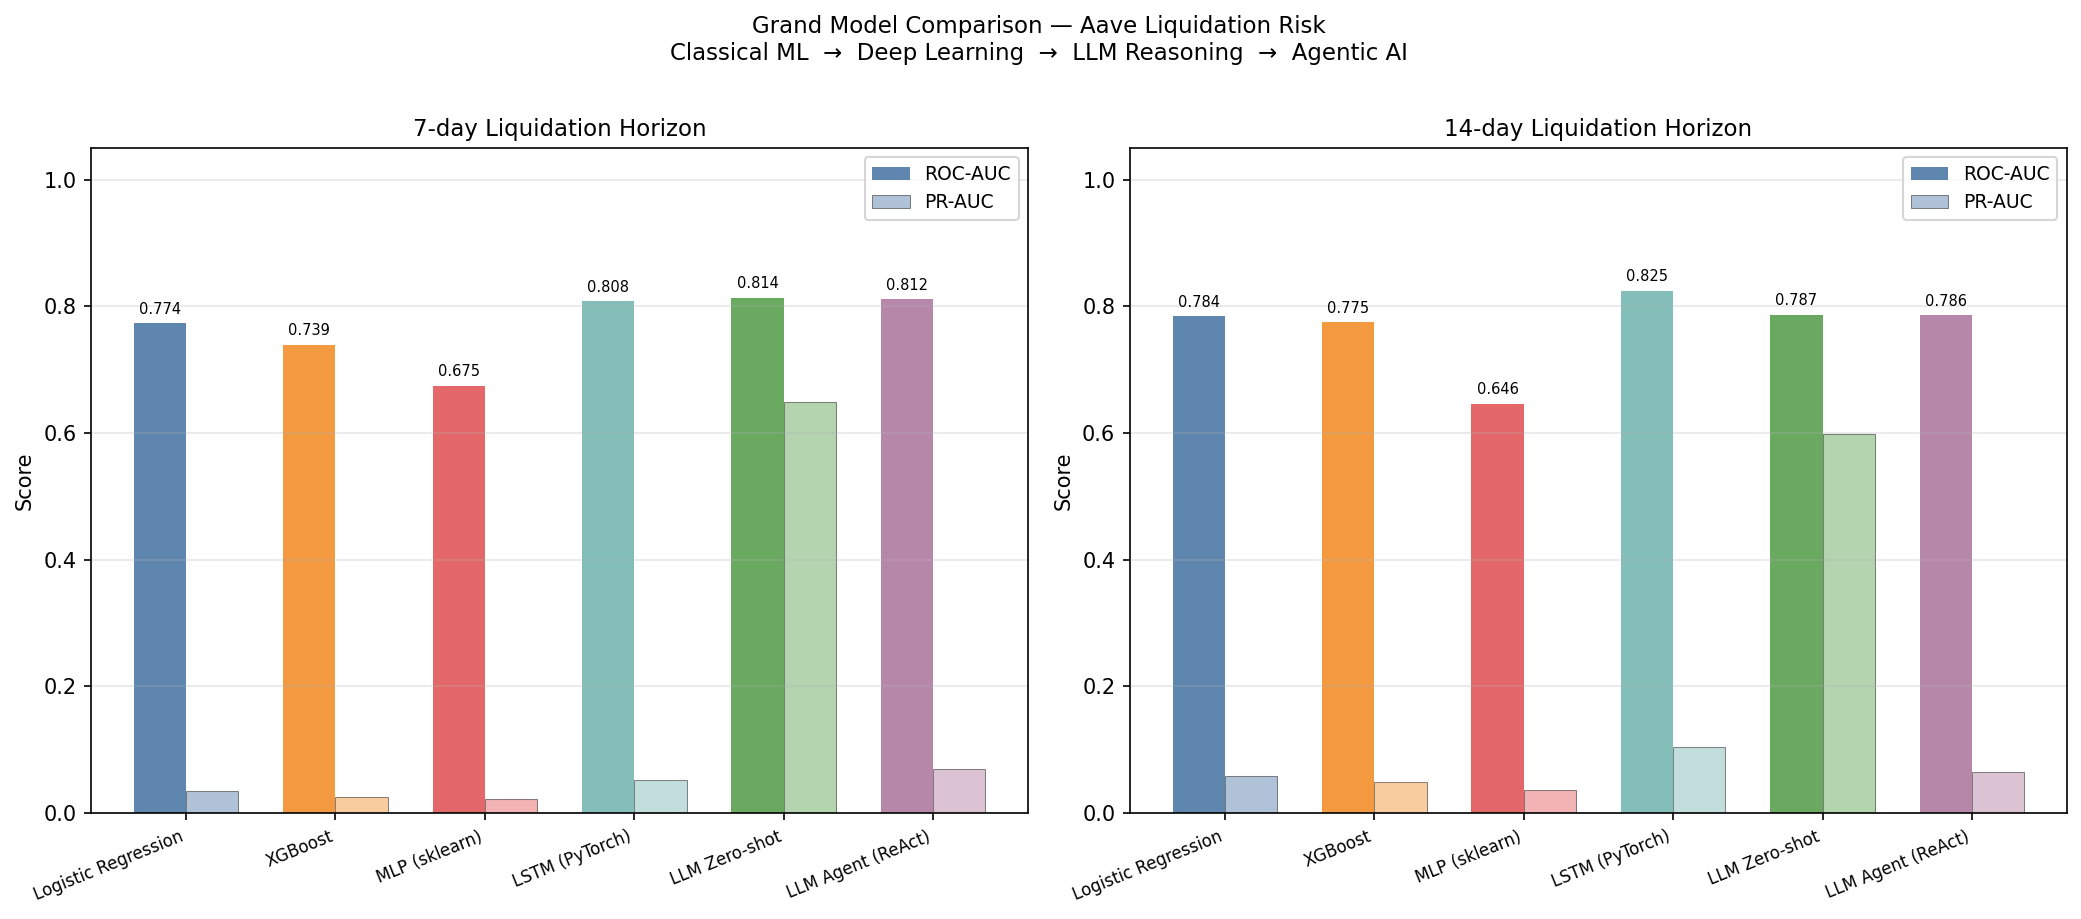
\includegraphics[width=\textwidth]{results/grand_comparison.png}
\caption{Grand comparison of ROC-AUC, PR-AUC, and Brier score across all
models and horizons.  PR-AUC values for LLM models (33\%-positive sample)
are not on the same scale as supervised-model values.}
\label{fig:grand}
\end{figure}

\subsection{ROC and Precision-Recall Curves}

Figure~\ref{fig:roc_pr} plots the ROC and precision-recall curves for
supervised models on the true-base-rate test set (7-day horizon).

\begin{figure}[htbp]
\centering
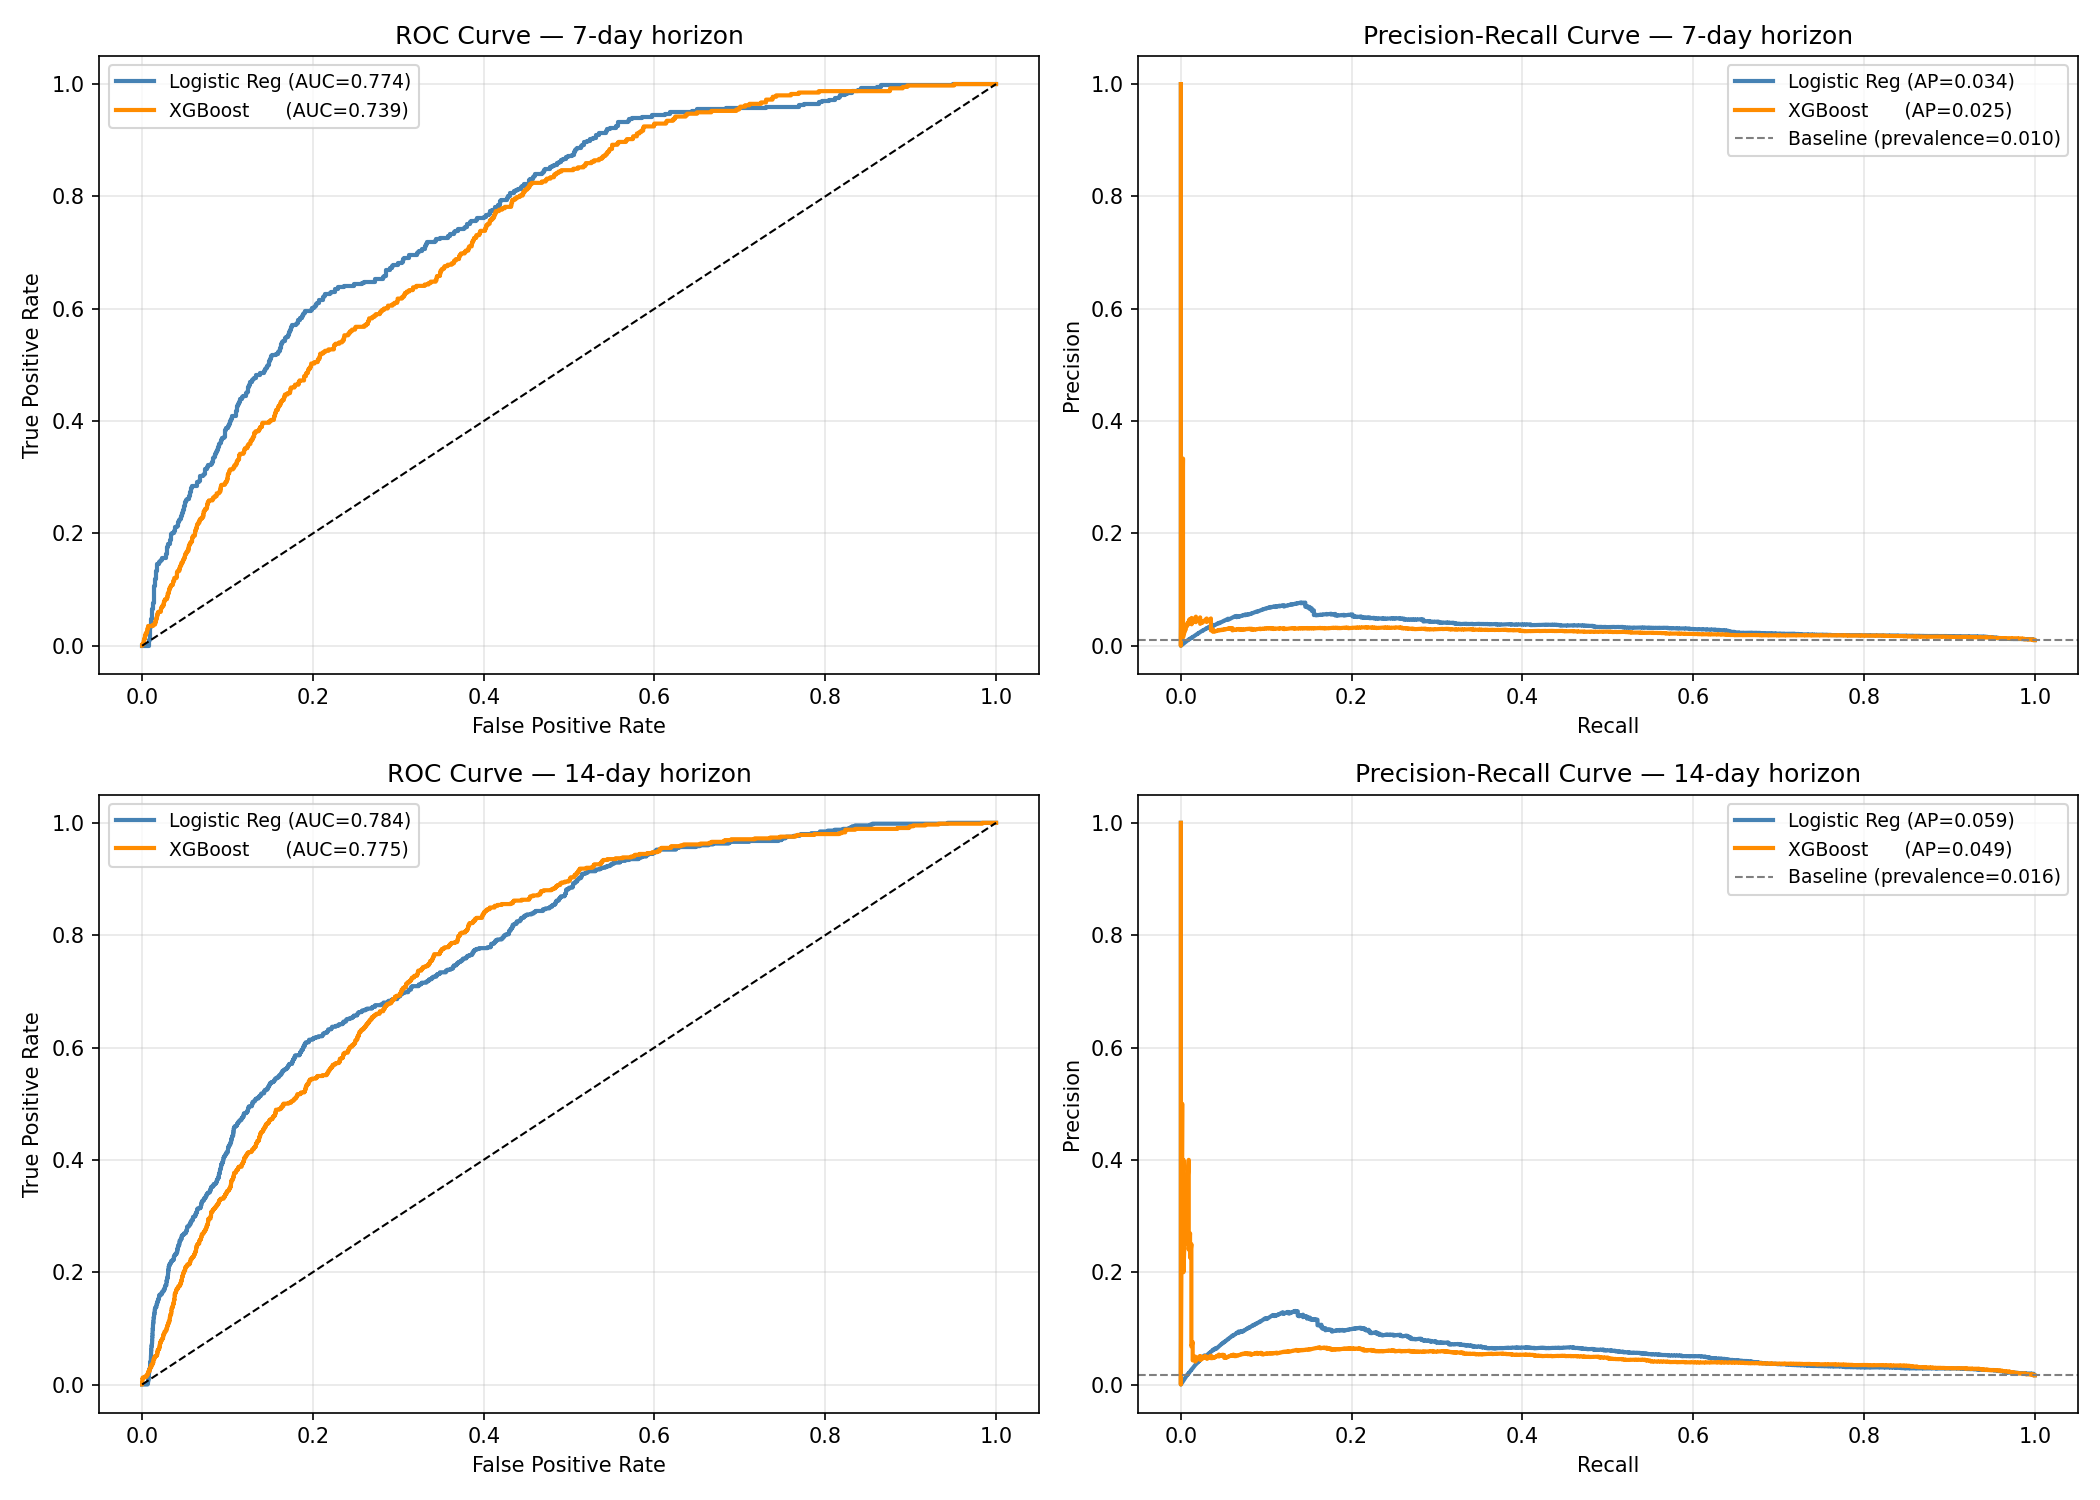
\includegraphics[width=\textwidth]{results/roc_pr_curves.png}
\caption{ROC curves (left) and precision-recall curves (right) for supervised
models on the held-out test set.  7-day horizon shown.}
\label{fig:roc_pr}
\end{figure}

\subsection{Discussion of Results}

The first question the table answers is whether sequence structure helps.
It does: the LSTM (ROC-AUC 0.809\,/\,0.825) outperforms all three
cross-sectional supervised models on both horizons by a consistent margin.
The gap between the LSTM and logistic regression---roughly 3.5 percentage
points on 7d---is not enormous, but it is reproducible and directionally
unambiguous.  An account whose health factor has been sliding downward for
three weeks carries different risk from one that arrived at the same current
HF after a brief volatility spike; a snapshot-based model sees both as
identical.

The second and more surprising pattern concerns the relative ordering of
the cross-sectional models.  Logistic regression (0.774\,/\,0.784) beats
XGBoost (0.739\,/\,0.775) on both horizons---a result that runs against the
conventional wisdom that gradient-boosted trees dominate tabular benchmarks.
The interpretation is that the dominant risk signal, proximity to the
liquidation boundary, is nearly linear in the log-odds.  XGBoost's capacity
to learn non-linear interactions adds little when those interactions are
either absent or too rare, given a 1\% positive rate, for the model to
reliably estimate them.  This changes slightly at the 14-day horizon, where
XGBoost gains 3.6 points and closes the gap, suggesting that additional
positive examples let the tree model begin to exploit second-order structure.
The MLP (0.675\,/\,0.646) sits at the bottom: without a sequence window and
with no structural advantage over LR in the linear regime, it is
outcompeted from both sides.

Across all models, the 14-day horizon is uniformly easier than 7-day,
consistent with more labelled positives (1.75\% vs.\ 1.08\%) and longer
run-up time for position features to reflect deteriorating conditions.

On calibration (Figure~\ref{fig:calibration}), Platt scaling and temperature
scaling bring logistic regression and the LSTM close to the diagonal.
XGBoost is the most overconfident model: predicted probabilities above 0.3
correspond to actual positive rates well below 0.1, which is why its Brier
score (0.050 on 7d) is five times that of the LSTM despite a smaller
ROC-AUC gap.

\begin{figure}[htbp]
\centering
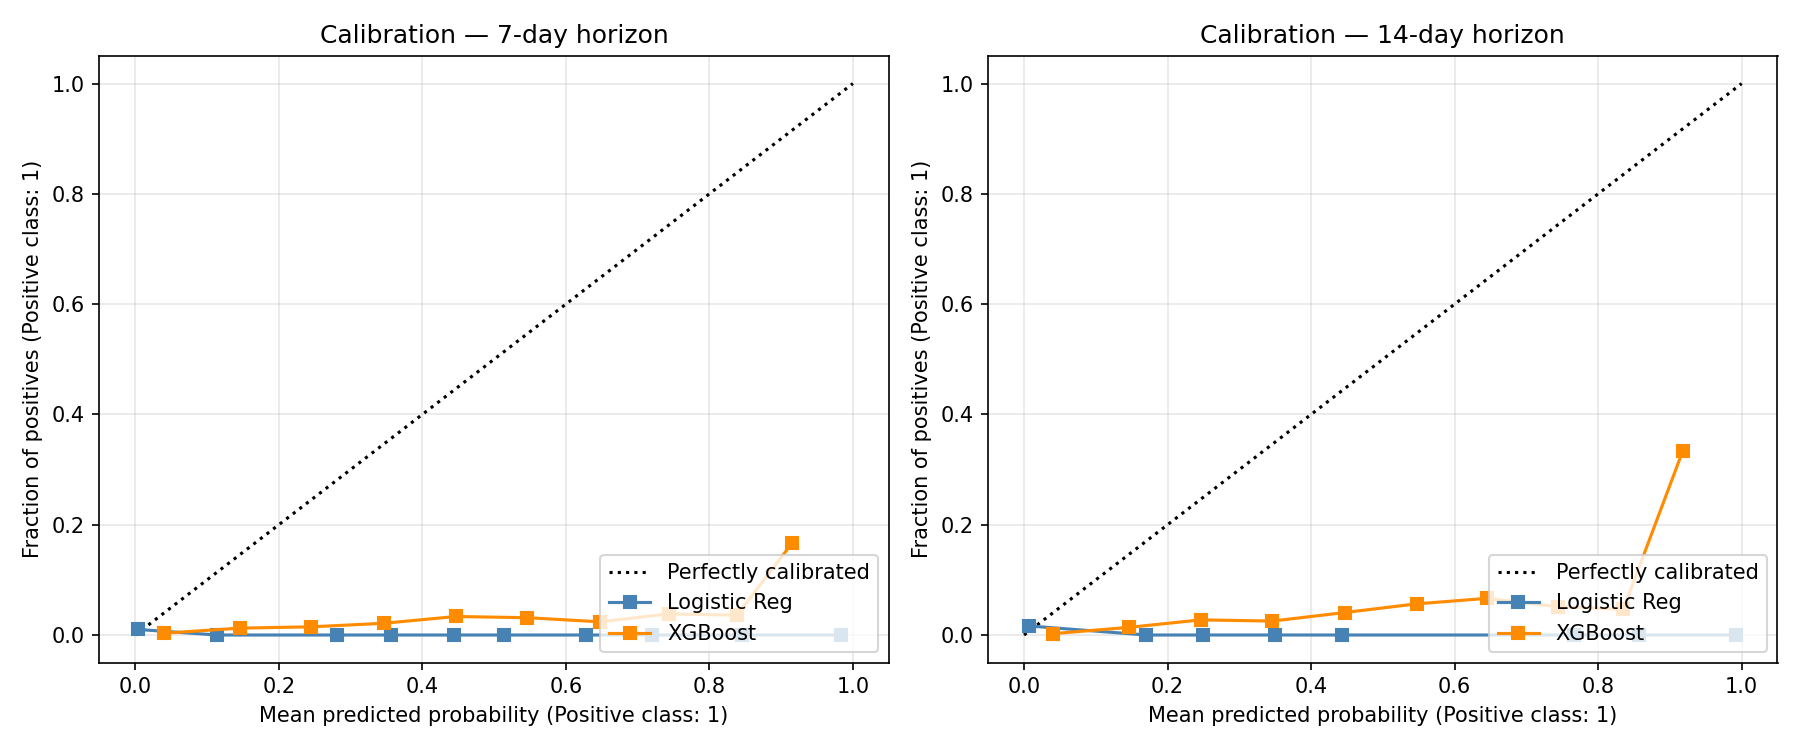
\includegraphics[width=0.88\textwidth]{results/calibration_curves.png}
\caption{Reliability diagrams for supervised models.  The diagonal represents
perfect calibration.  Platt-scaled LR and temperature-scaled LSTM come
closest; XGBoost is notably overconfident at high predicted probabilities.}
\label{fig:calibration}
\end{figure}

\subsection{Regime Analysis}

Figure~\ref{fig:regime} breaks down ROC-AUC into high- and low-volatility
periods (split at the median of \texttt{realized\_vol\_7d}).  All models
discriminate better during high-volatility regimes, which is intuitive:
sharp price movements push marginal accounts across the liquidation boundary
more decisively, creating cleaner positive examples.

\begin{figure}[htbp]
\centering
\begin{subfigure}[b]{0.48\textwidth}
    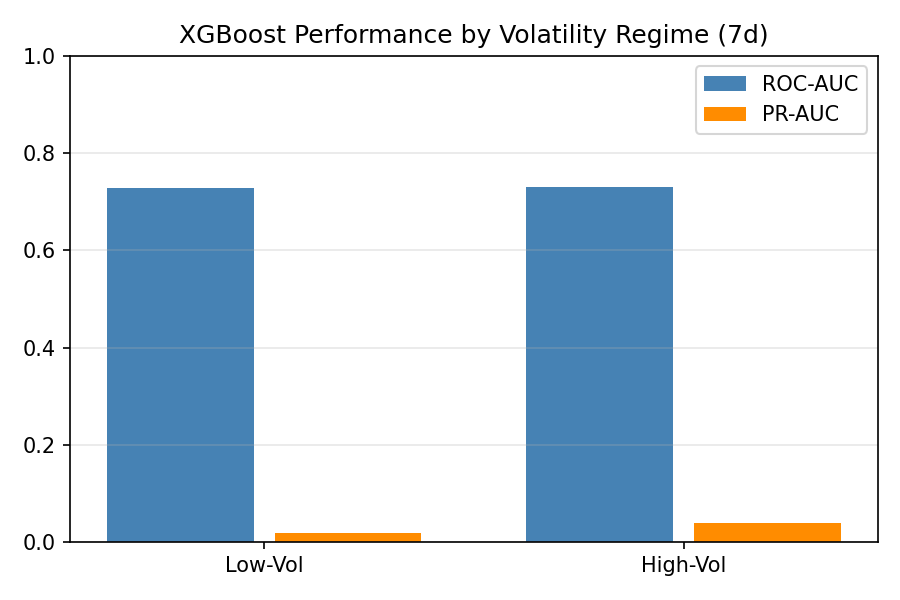
\includegraphics[width=\textwidth]{results/regime_comparison_7d.png}
    \caption{7-day horizon}
\end{subfigure}
\begin{subfigure}[b]{0.48\textwidth}
    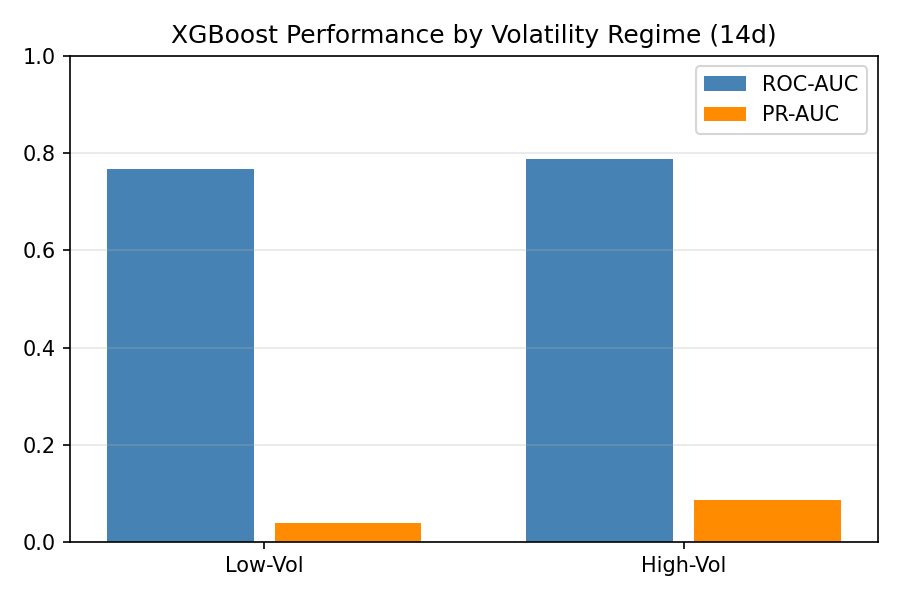
\includegraphics[width=\textwidth]{results/regime_comparison_14d.png}
    \caption{14-day horizon}
\end{subfigure}
\caption{ROC-AUC by market regime (high- vs.\ low-volatility).  Higher
volatility improves discrimination across all models on both horizons.}
\label{fig:regime}
\end{figure}
% ============================================================
\section{Interpretability Analysis}
\label{sec:interpretability}
% ============================================================

We apply SHAP TreeExplainer to the XGBoost model and partial dependence
plots to both logistic regression and XGBoost.

\subsection{Global SHAP Importance}

\begin{figure}[htbp]
\centering
\begin{subfigure}[b]{0.48\textwidth}
    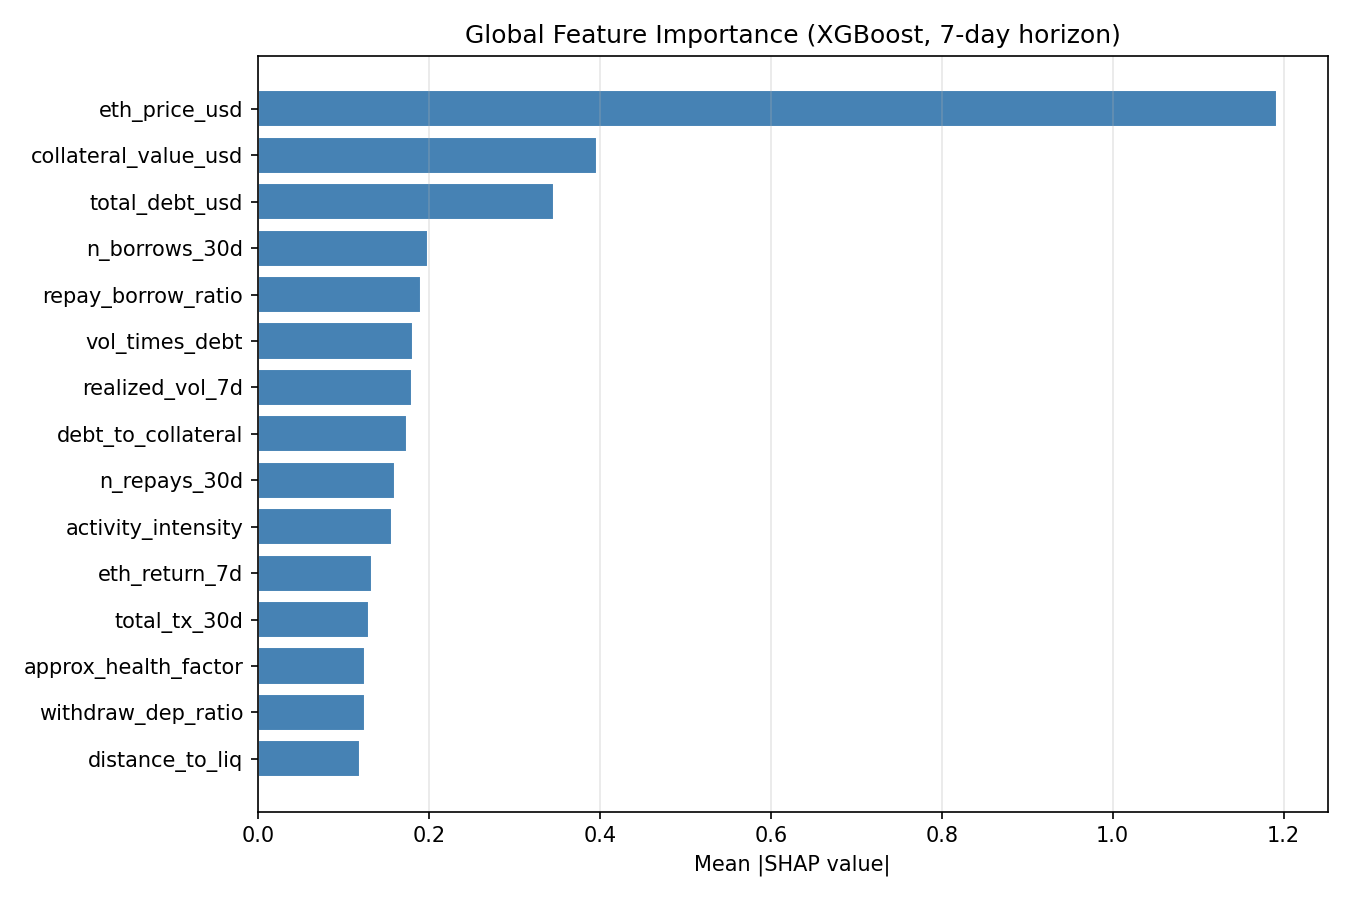
\includegraphics[width=\textwidth]{results/shap_global_7d.png}
    \caption{7-day horizon}
\end{subfigure}
\hfill
\begin{subfigure}[b]{0.48\textwidth}
    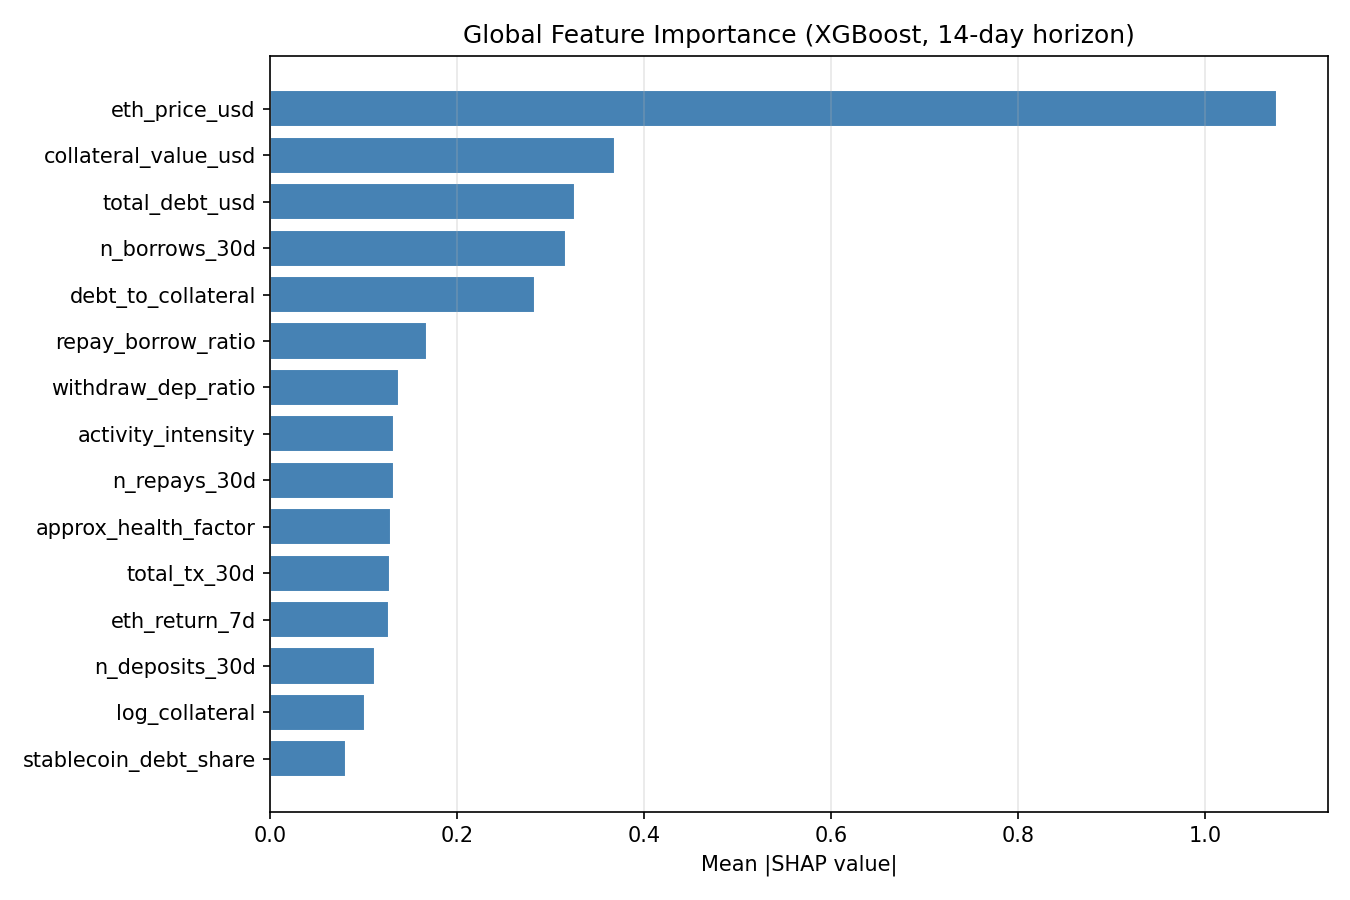
\includegraphics[width=\textwidth]{results/shap_global_14d.png}
    \caption{14-day horizon}
\end{subfigure}
\caption{Mean absolute SHAP values (global feature importance) for XGBoost.
Rankings are stable across both horizons.}
\label{fig:shap_global}
\end{figure}

\texttt{approx\_health\_factor} and \texttt{distance\_to\_liq} rank first and
second on both horizons.  The two features encode the same underlying
quantity---proximity to the liquidation boundary---through different scales
(a ratio vs.\ an absolute difference), and their joint dominance suggests
that most predictive signal concentrates in this single dimension of the
feature space.

\texttt{vol\_times\_debt} ranks consistently in the top five.  It captures
a natural interaction: a large debt position amplifies the dollar impact of
any given percentage move in collateral price.  \texttt{stablecoin\_debt\_share}
also appears: because stablecoin-denominated liabilities do not depreciate in
USD terms, a higher stablecoin share reduces the account's exposure to
collateral price swings.

\subsection{SHAP Beeswarm Plots}

\begin{figure}[htbp]
\centering
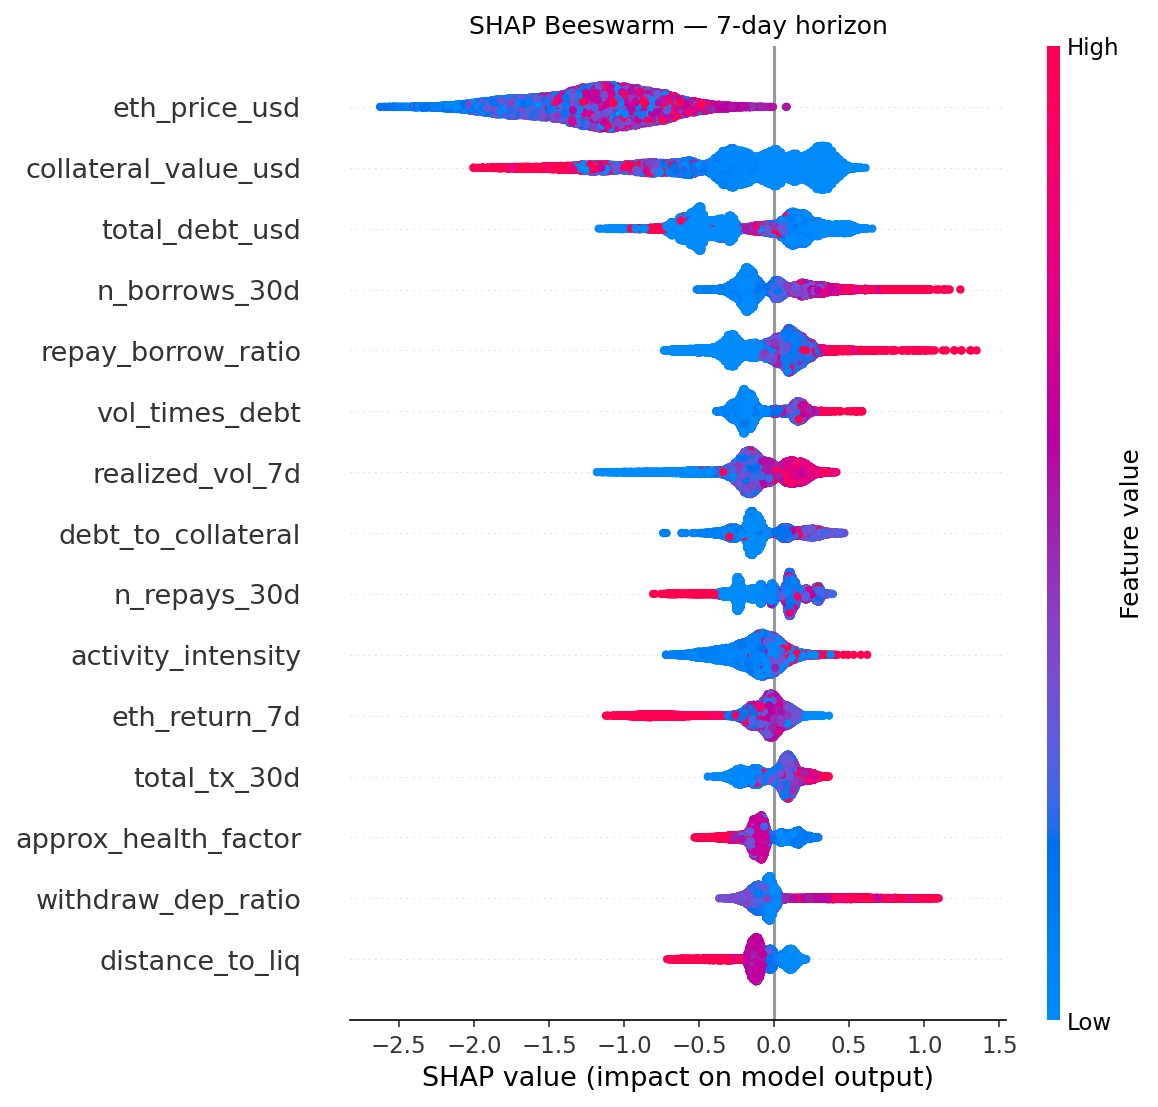
\includegraphics[width=\textwidth]{results/shap_beeswarm_7d.png}
\caption{SHAP beeswarm plot, 7-day horizon.  Each point is one test
observation, coloured red (high feature value) or blue (low feature value).
Position on the horizontal axis shows the signed contribution to the
log-odds prediction.}
\label{fig:shap_beeswarm_7d}
\end{figure}

\begin{figure}[htbp]
\centering
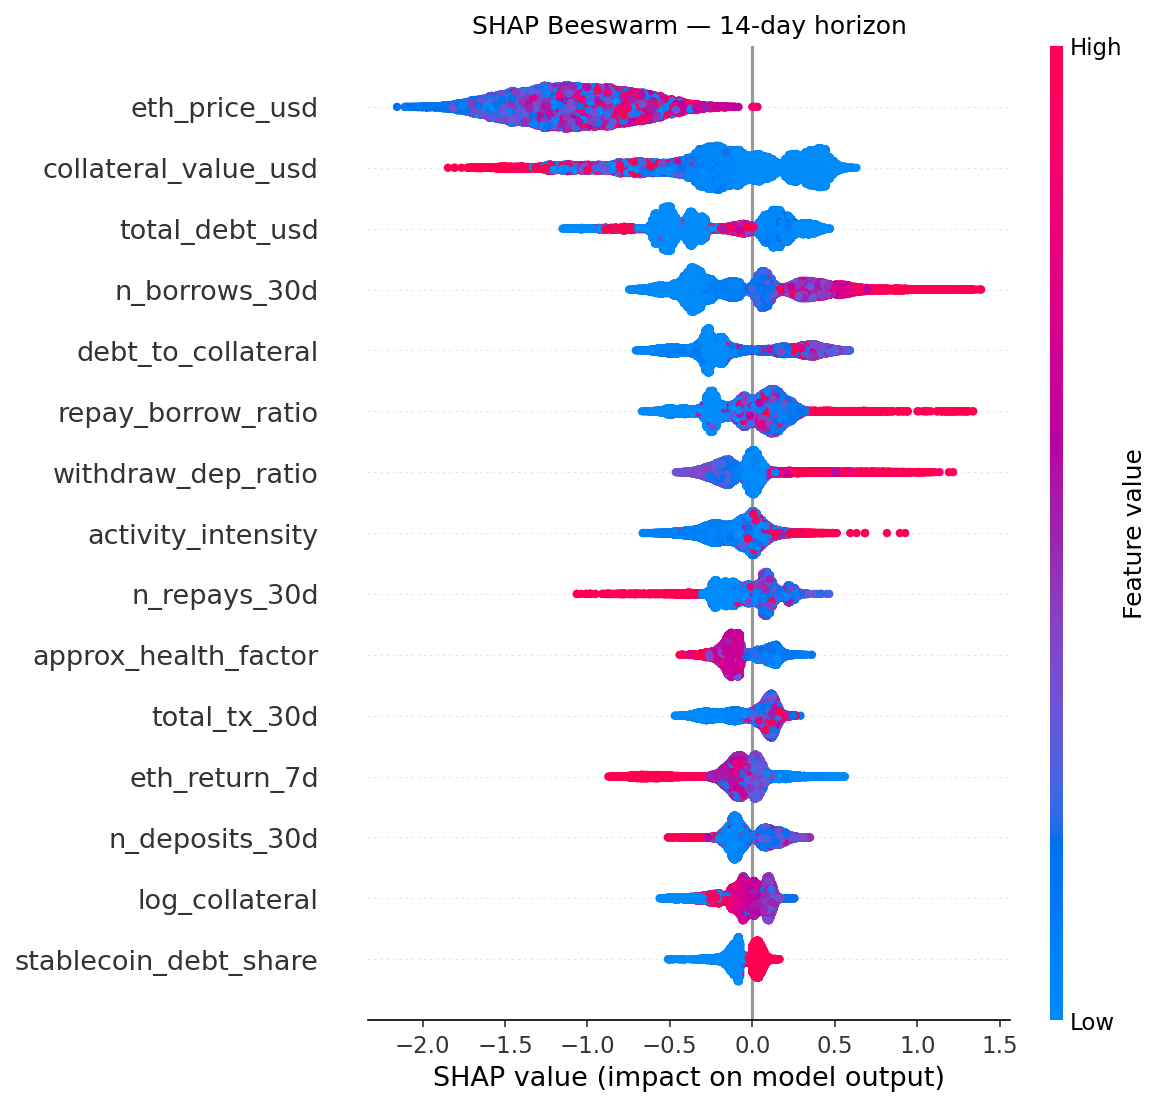
\includegraphics[width=\textwidth]{results/shap_beeswarm_14d.png}
\caption{SHAP beeswarm plot, 14-day horizon.  Colour and axis conventions
as in the 7-day panel above.}
\label{fig:shap_beeswarm_14d}
\end{figure}

Three patterns stand out in Figures~\ref{fig:shap_beeswarm_7d}--\ref{fig:shap_beeswarm_14d}:

\begin{itemize}[noitemsep]
    \item \textbf{\texttt{approx\_health\_factor}}: the effect is highly
    non-linear.  Accounts with HF near 1 (blue) accumulate large positive
    SHAP values; the contribution decays toward zero well before HF reaches 3.
    This means that once an account is ``safe enough'', further increases in
    its buffer have no practical effect on the model's output.
    \item \textbf{\texttt{eth\_return\_7d}}: recent negative returns (blue)
    push the prediction toward liquidation, as expected given that most
    collateral on Aave V2 is ETH or ETH-correlated.
    \item \textbf{\texttt{repay\_borrow\_ratio}}: high repayment activity
    (red) is associated with \emph{higher} predicted liquidation probability,
    not lower.  This counter-intuitive finding---repaying more means higher
    risk---is consistent with a behavioural signature of distress: accounts
    that are rapidly deleveraging are likely already aware that their position
    is dangerously close to the threshold.
\end{itemize}

\subsection{Instance-Level Explanation}

Figure~\ref{fig:waterfall} shows SHAP waterfall decompositions for a
representative high-risk account.  Starting from the model's baseline
prediction, each bar shows how much a single feature shifts the output.
Low health factor and high \texttt{vol\_times\_debt} together account for
most of the uplift above the base rate.

\begin{figure}[htbp]
\centering
\begin{subfigure}[b]{0.95\textwidth}
    \centering
    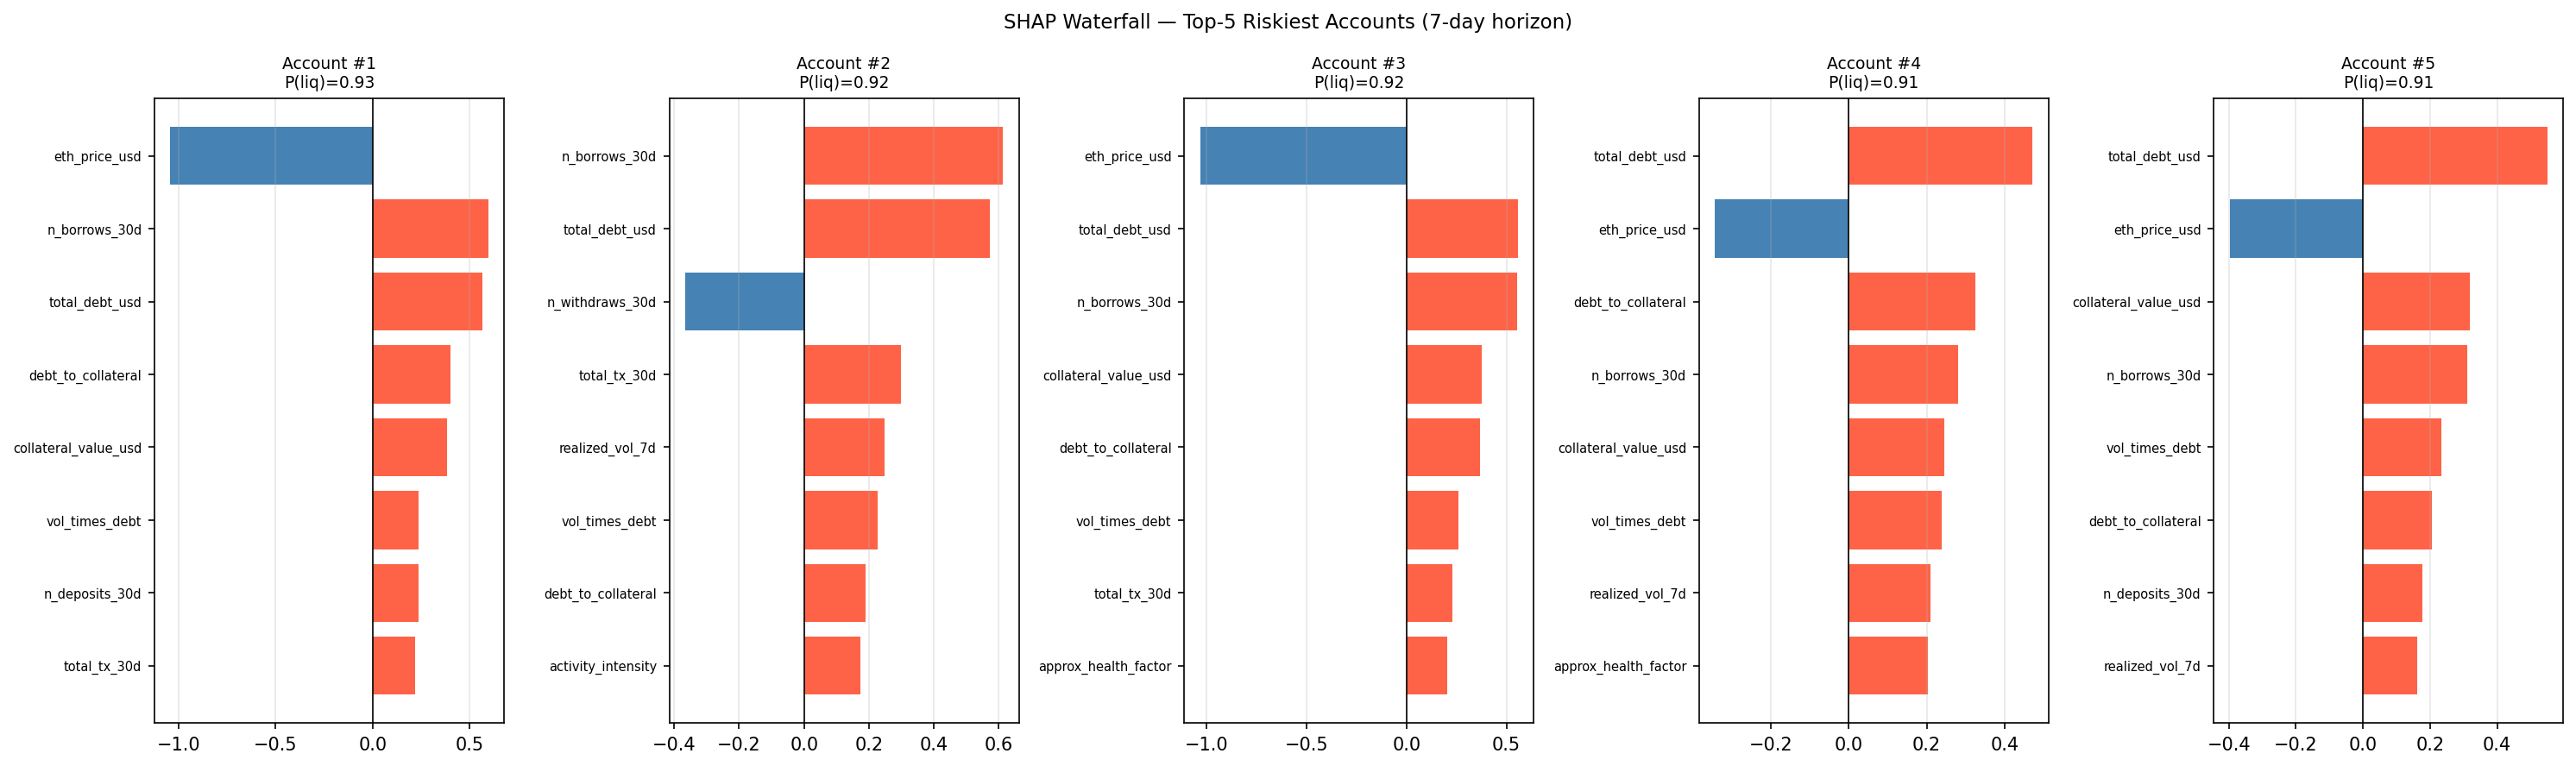
\includegraphics[width=\textwidth]{results/shap_waterfall_7d.png}
    \caption{7-day horizon}
\end{subfigure}
\hfill
\begin{subfigure}[b]{0.95\textwidth}
    \centering
    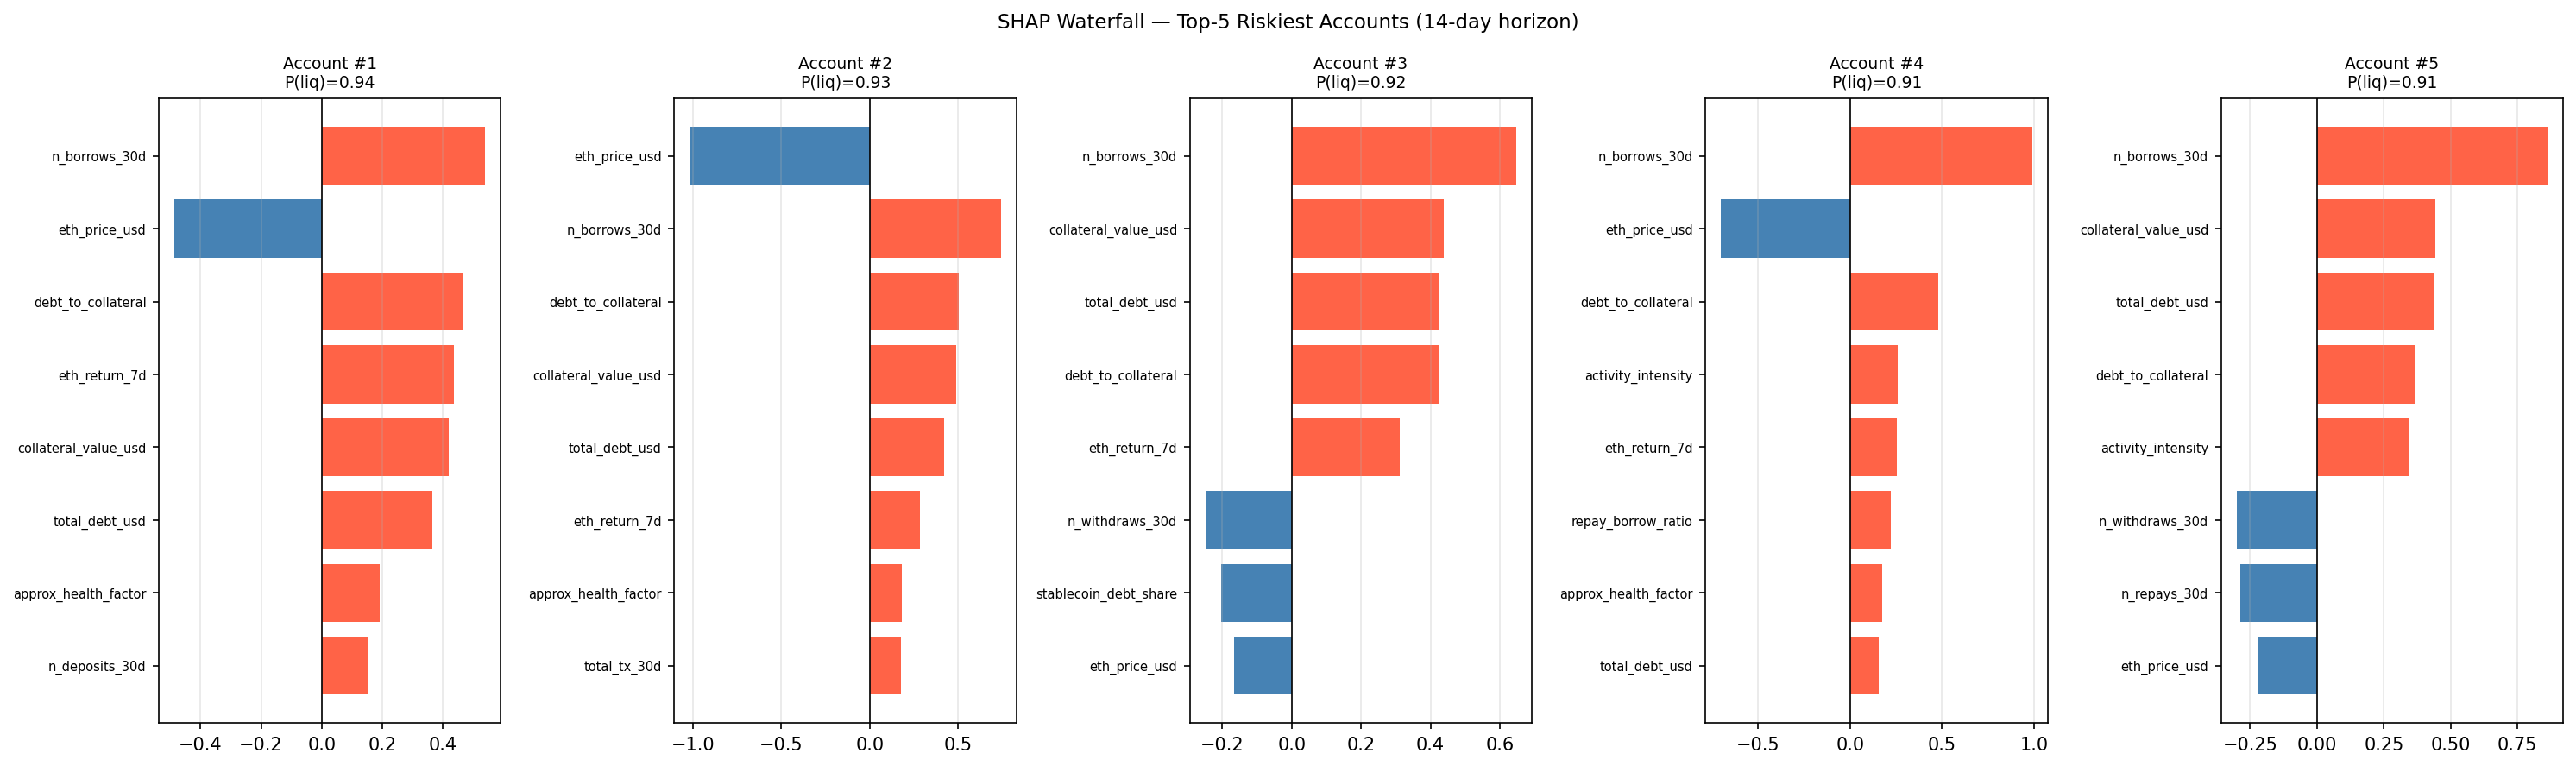
\includegraphics[width=\textwidth]{results/shap_waterfall_14d.png}
    \caption{14-day horizon}
\end{subfigure}
\caption{SHAP waterfall charts for a representative high-risk account,
decomposing the model's prediction into additive feature contributions.}
\label{fig:waterfall}
\end{figure}

\subsection{Partial Dependence Plots}

\begin{figure}[htbp]
\centering
\begin{subfigure}[b]{0.48\textwidth}
    \centering
    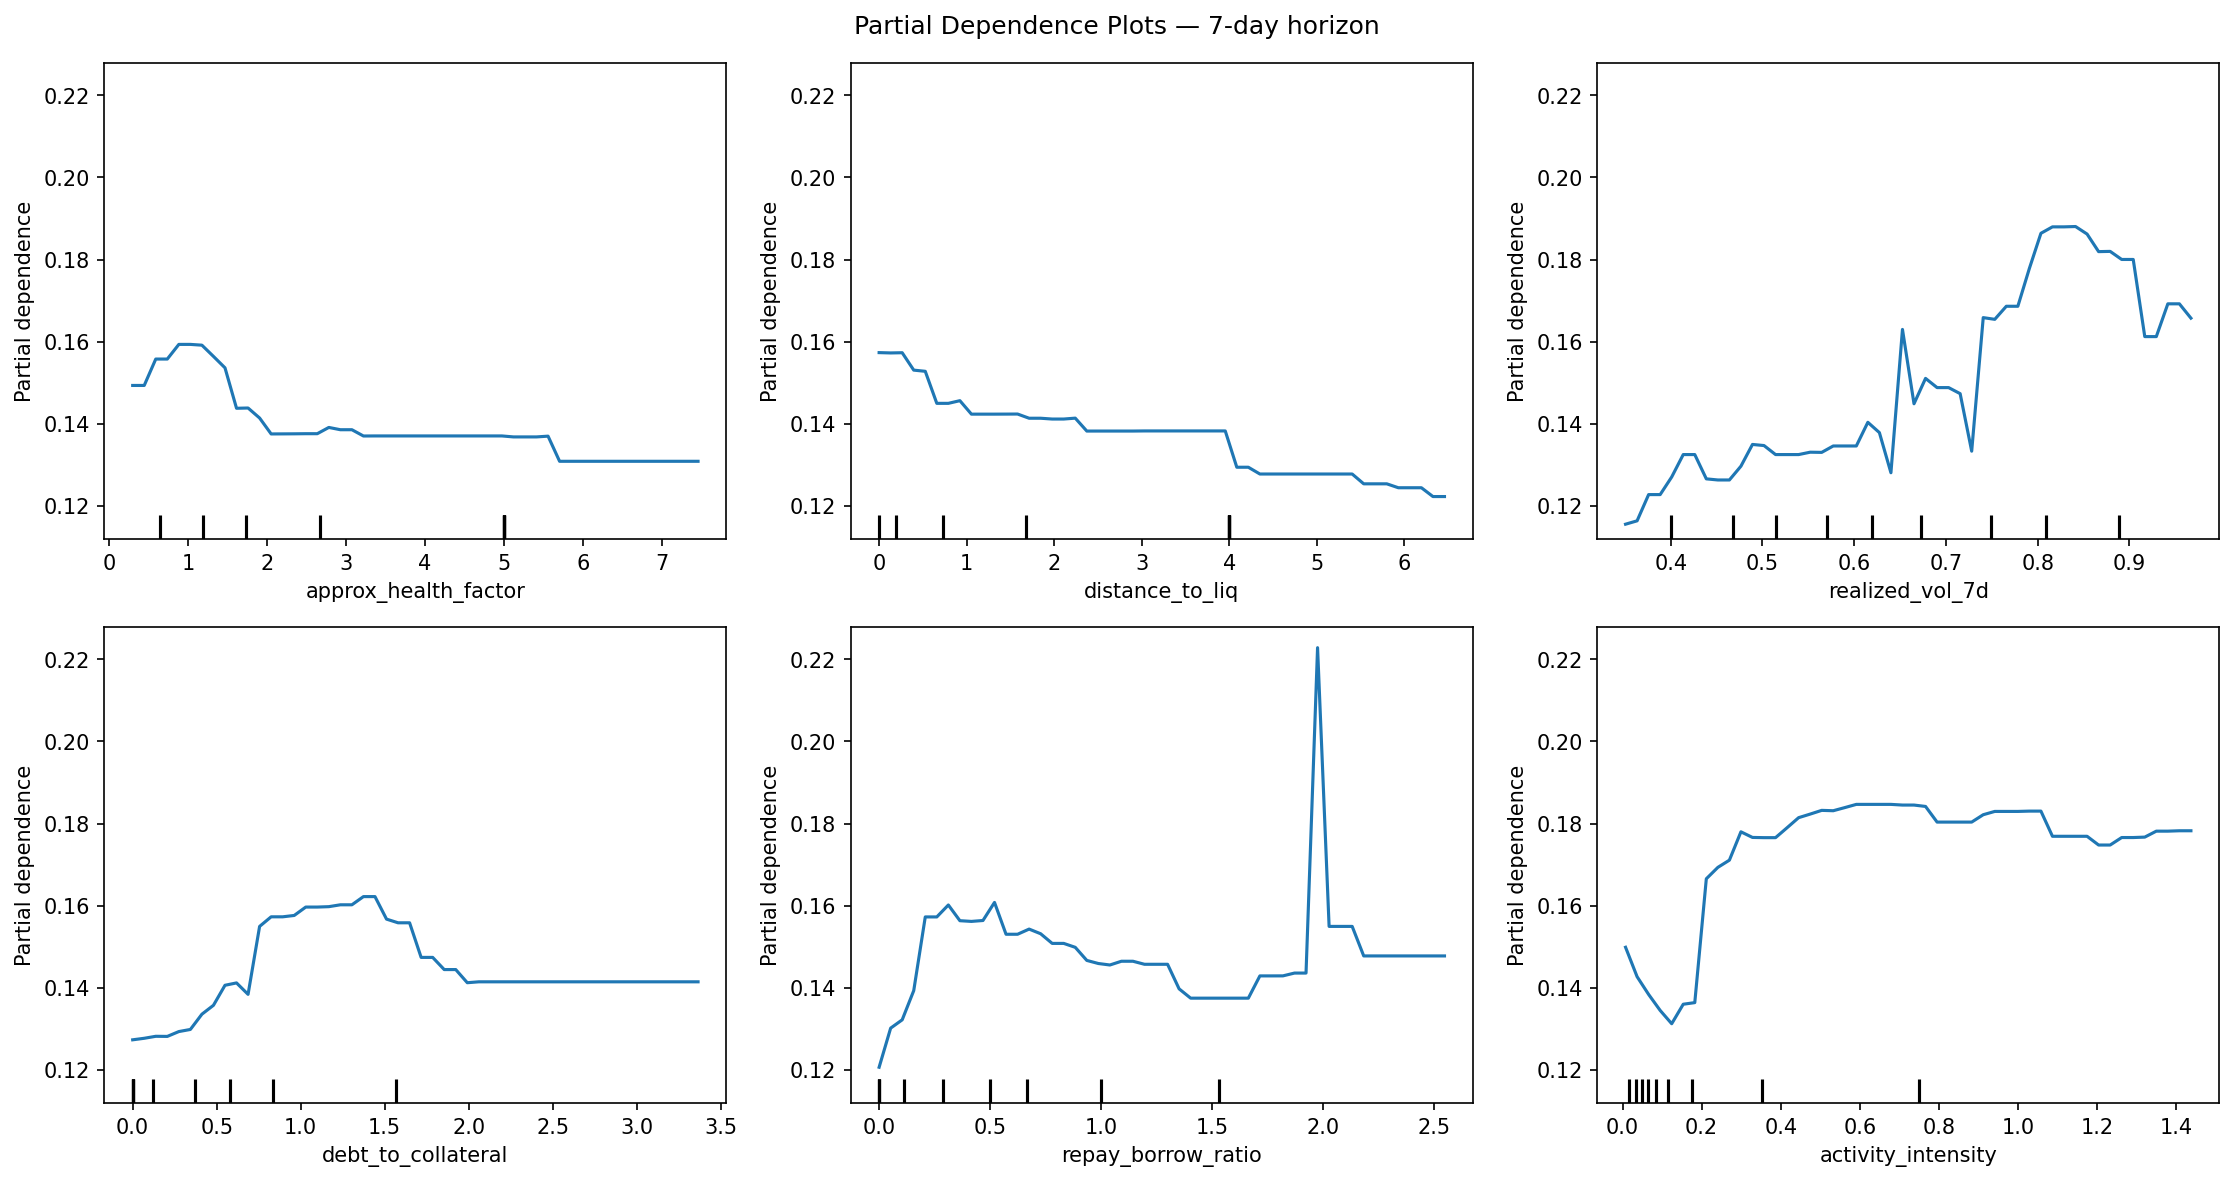
\includegraphics[width=\textwidth]{results/pdp_1d_7d.png}
    \caption{7-day horizon}
\end{subfigure}
\hfill
\begin{subfigure}[b]{0.48\textwidth}
    \centering
    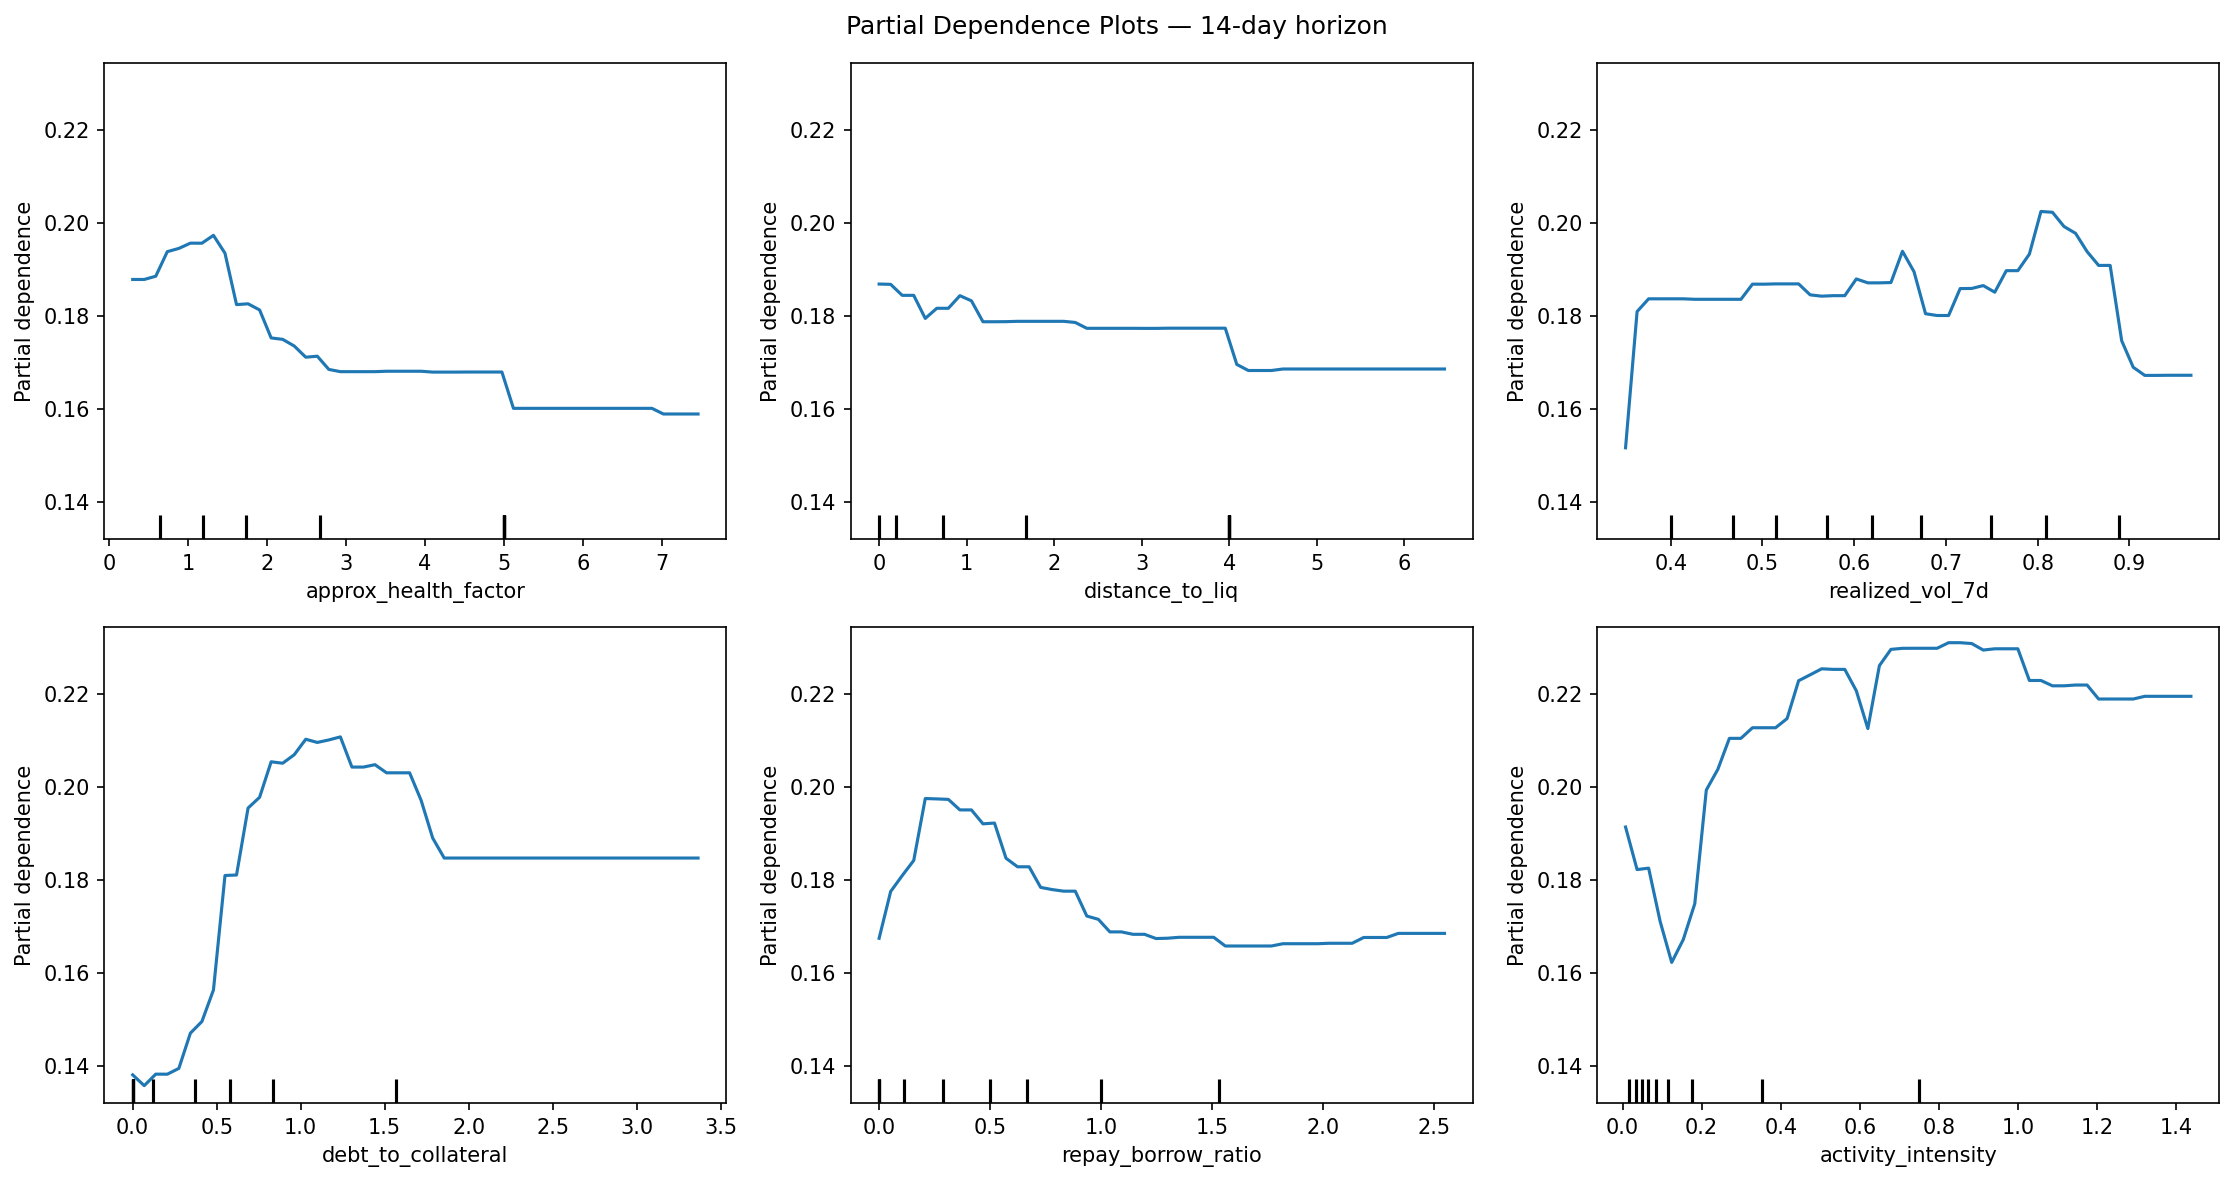
\includegraphics[width=\textwidth]{results/pdp_1d_14d.png}
    \caption{14-day horizon}
\end{subfigure}
\caption{1-D partial dependence plots for the top features.  Each curve
shows the marginal effect of that feature, averaged over the full test set.}
\label{fig:pdp_1d}
\end{figure}

\begin{figure}[htbp]
\centering
\begin{subfigure}[b]{0.47\textwidth}
    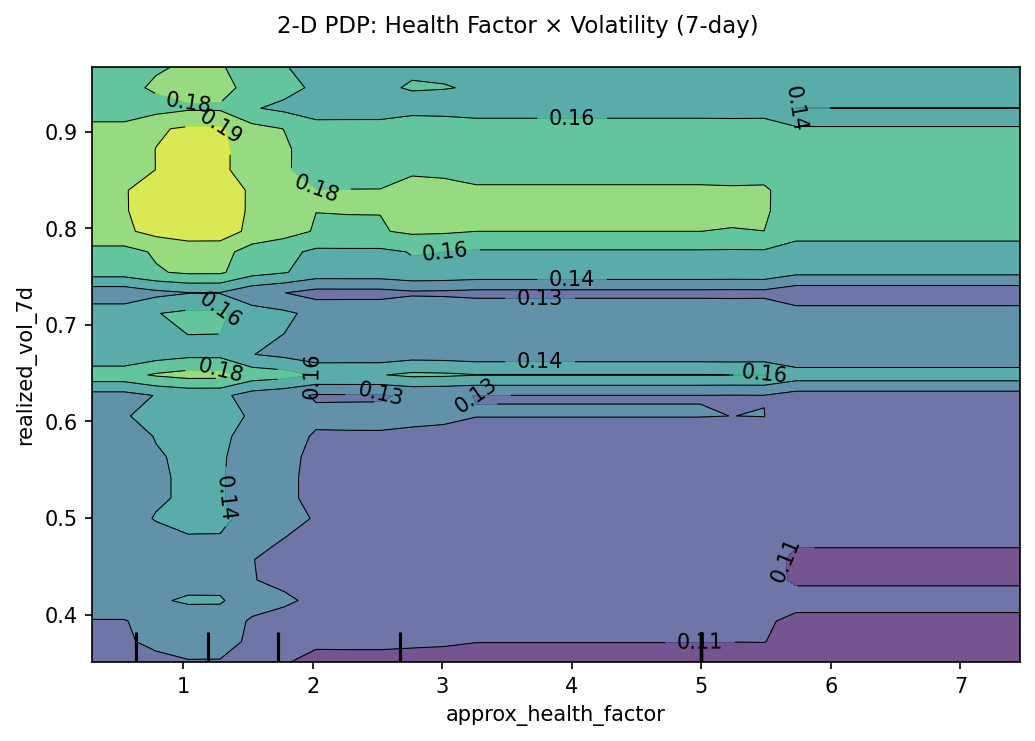
\includegraphics[width=\textwidth]{results/pdp_2d_hf_vol_7d.png}
    \caption{7-day horizon}
\end{subfigure}
\hfill
\begin{subfigure}[b]{0.47\textwidth}
    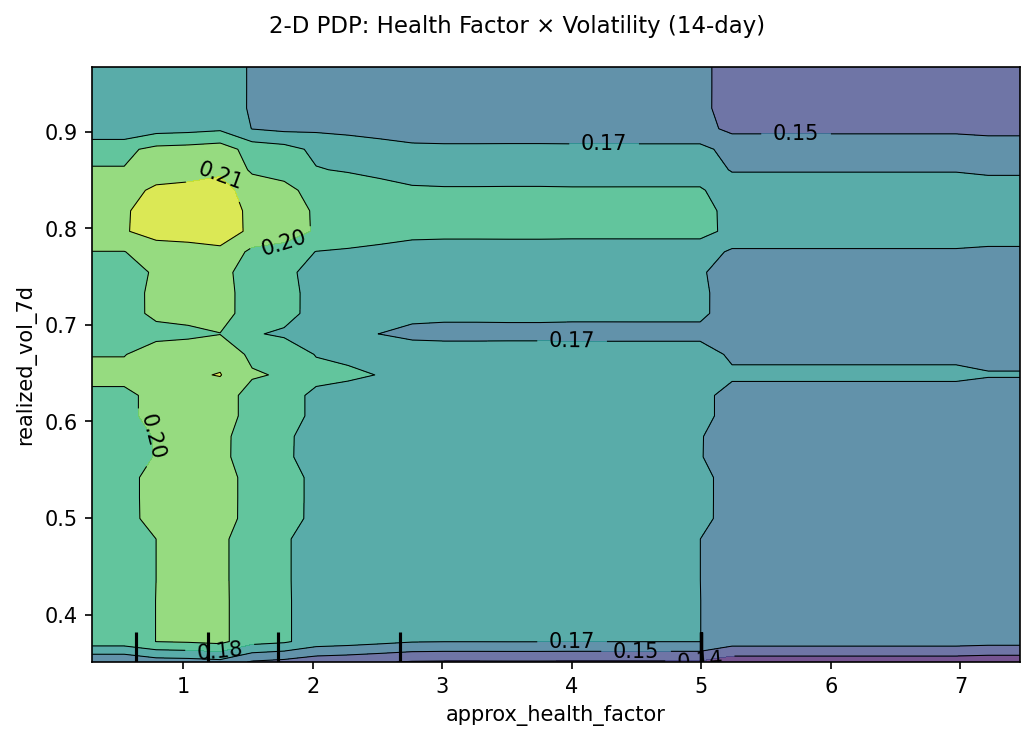
\includegraphics[width=\textwidth]{results/pdp_2d_hf_vol_14d.png}
    \caption{14-day horizon}
\end{subfigure}
\caption{2-D partial dependence: health factor vs.\ realised volatility.
Risk is highest in the low-HF, high-volatility corner (top-left), confirming
that market turbulence amplifies position vulnerability.}
\label{fig:pdp_2d}
\end{figure}

The 2-D PDP in Figure~\ref{fig:pdp_2d} shows that the volatility effect
is concentrated at low health factors.  For accounts with HF $> 3$, even
elevated volatility contributes little to predicted liquidation probability.
The interaction is thus not simply additive but exhibits a threshold
character: volatility matters primarily when the position is already under
stress.

\clearpage

% ============================================================
\section{Survival Analysis}
\label{sec:survival}
% ============================================================

\subsection{Kaplan--Meier Survival Curves}

\begin{figure}[htbp]
\centering
\begin{subfigure}{\textwidth}
    \centering
    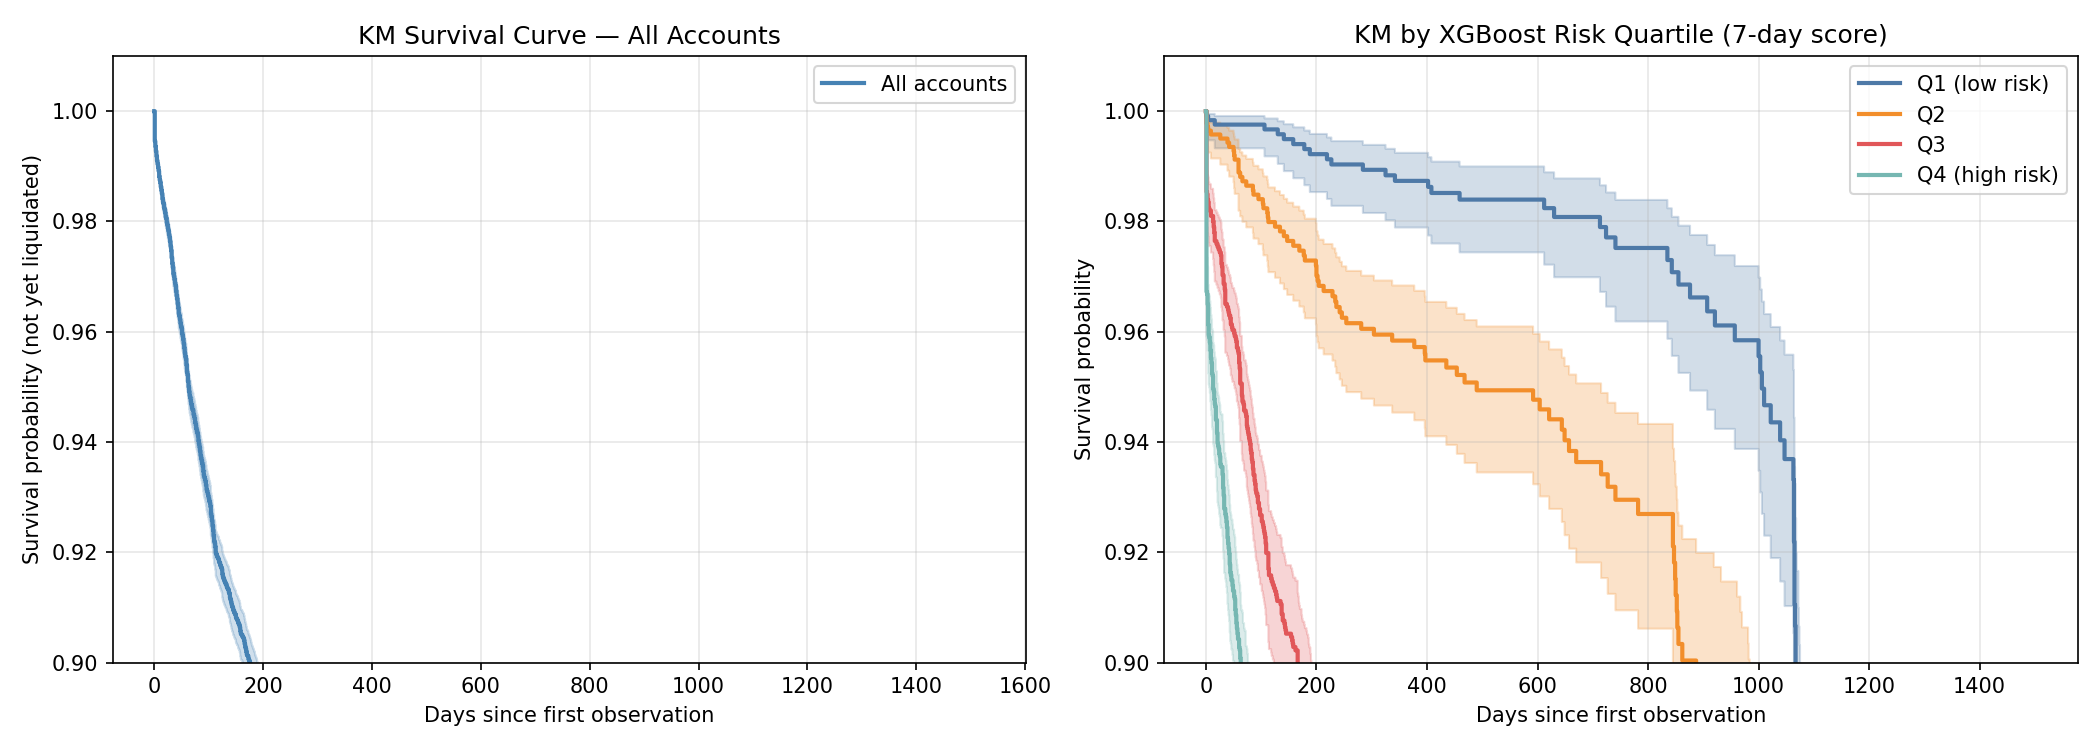
\includegraphics[width=\textwidth]{results/km_curves_7d.png}
    \caption{7-day horizon}
\end{subfigure}
\vspace{0.4em}
\begin{subfigure}{\textwidth}
    \centering
    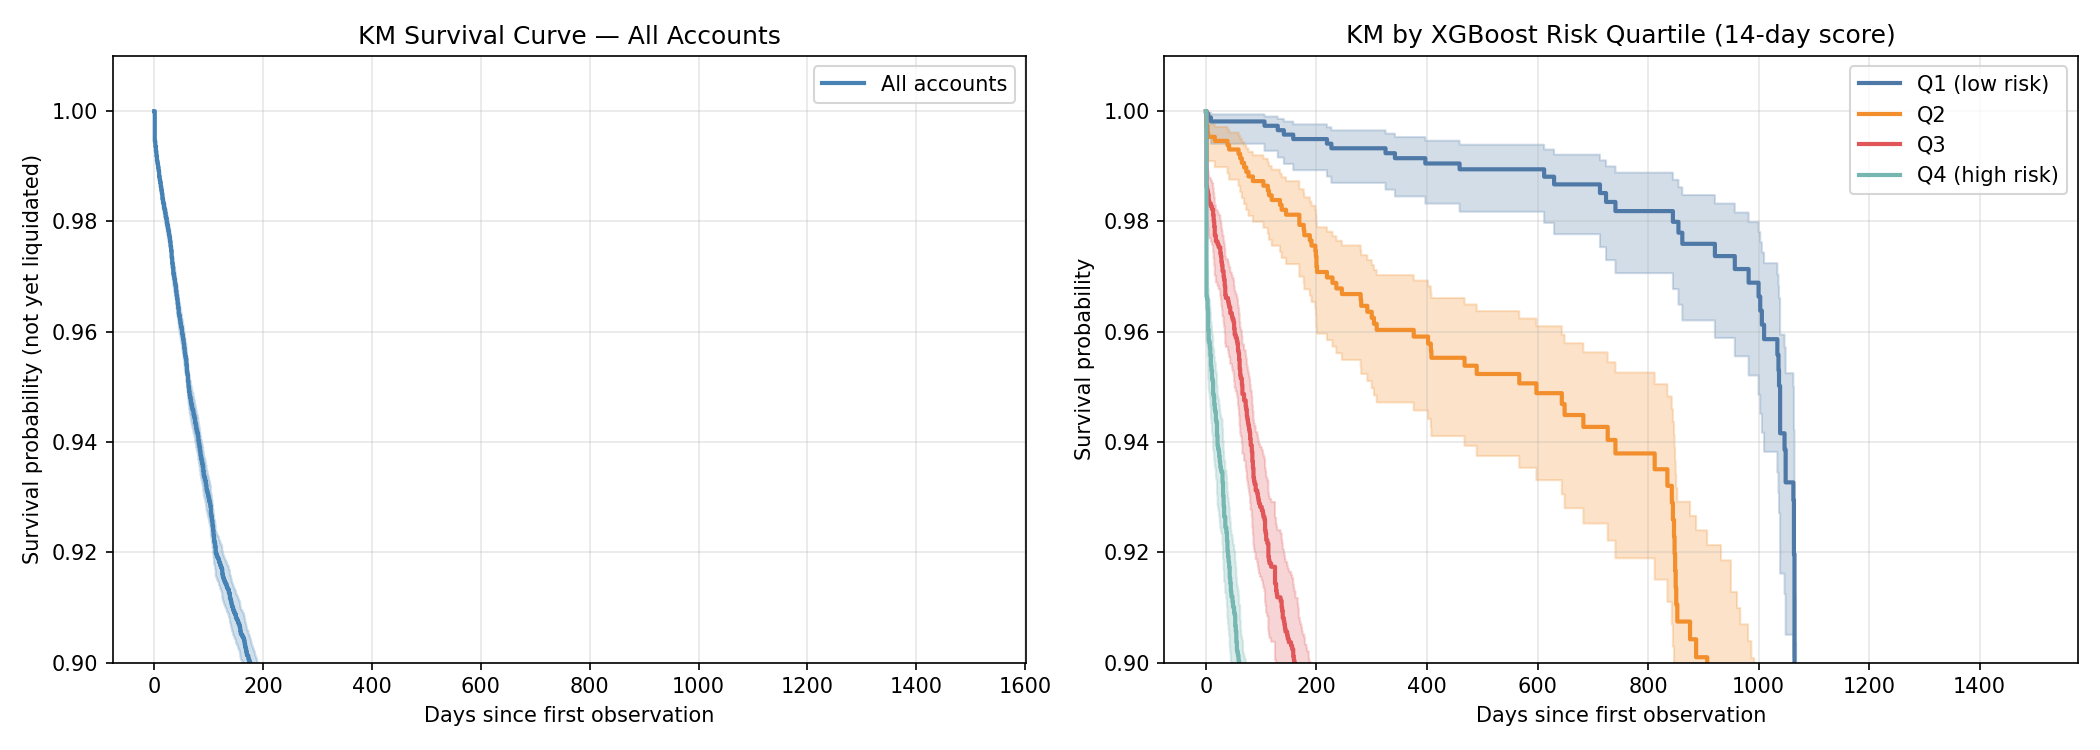
\includegraphics[width=\textwidth]{results/km_curves_14d.png}
    \caption{14-day horizon}
\end{subfigure}
\caption{Kaplan--Meier survival curves stratified by initial health factor
quintile.  Shaded bands are 95\% confidence intervals.  Log-rank
$p \ll 0.001$ on both horizons.}
\label{fig:km}
\end{figure}

Figure~\ref{fig:km} shows that accounts in the lowest HF quintile face
dramatically higher liquidation hazard from the very first observation day,
and the gap widens over time.  The confidence intervals for the high-HF
strata remain narrow and close to one even out to 30 days, confirming that
well-collateralised accounts rarely encounter liquidation within short windows.

\subsection{Stratified Cox Proportional Hazards}

Table~\ref{tab:cox} reports estimated hazard ratios.  The model is
stratified by quartile bins of \texttt{realized\_vol\_7d} and
\texttt{repay\_borrow\_ratio} to account for the non-proportional effects
identified by Schoenfeld residuals.

\begin{table}[htbp]
\centering
\caption{Stratified Cox hazard ratios.  Strata: quartile bins of
\texttt{realized\_vol\_7d} and \texttt{repay\_borrow\_ratio}.
Harrell's C-index $= 0.691$; $N = 52{,}918$ accounts;
$n_\text{events} = 4{,}947$ (9.35\% event rate, pooled sample).}
\label{tab:cox}
\renewcommand{\arraystretch}{1.2}
\begin{tabular}{lccc}
\toprule
\textbf{Feature} & \textbf{Log HR} & \textbf{Hazard Ratio} & \textbf{Direction} \\
\midrule
\texttt{approx\_health\_factor}        & $-0.145$ & 0.865 & Protective \\
\texttt{distance\_to\_liq}             & $-0.130$ & 0.878 & Protective \\
\texttt{debt\_to\_collateral}          & $-0.001$ & 0.999 & Neutral \\
\texttt{stablecoin\_debt\_share}       & $+0.080$ & 1.084 & Risk factor \\
\texttt{eth\_return\_7d}               & $+0.021$ & 1.022 & Mild risk \\
\texttt{activity\_intensity}           & $-0.011$ & 0.989 & Mild protective \\
\texttt{realized\_vol\_7d}$^\dagger$   & $-0.081$ & 0.922 & (stratified) \\
\texttt{repay\_borrow\_ratio}$^\dagger$ & $+0.262$ & 1.300 & (stratified) \\
\bottomrule
\multicolumn{4}{l}{\small$^\dagger$ Strata variables; HR interpretation requires caution.}
\end{tabular}
\end{table}

\begin{figure}[htbp]
\centering
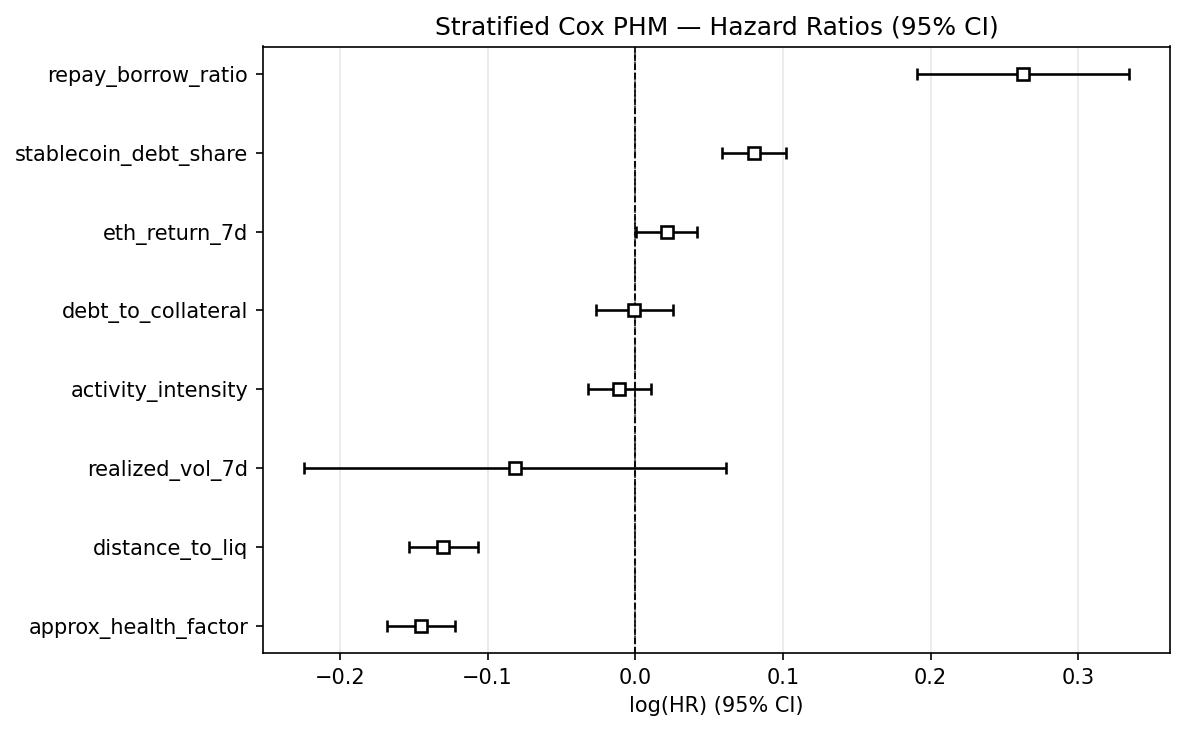
\includegraphics[width=0.85\textwidth]{results/cox_hazard_ratios.png}
\caption{Forest plot of Cox hazard ratios with 95\% confidence intervals.}
\label{fig:cox}
\end{figure}

Health factor and distance-to-liquidation are the strongest protective
factors, as expected: each additional unit of HF reduces the instantaneous
hazard by roughly 13\%.  \texttt{stablecoin\_debt\_share} acts as a mild
risk factor (HR 1.084).  One plausible mechanism is that accounts that
deliberately borrow stablecoins---for yield farming or leverage---tend to
run higher leverage ratios overall, accepting thinner safety margins in
exchange for yield.

The most striking finding is the hazard ratio of 1.300 on
\texttt{repay\_borrow\_ratio}.  Accounts with disproportionately high
repayment activity face 30\% higher instantaneous hazard, even controlling
for the current health factor.  This aligns with the SHAP findings above:
frantic repayment is a behavioural precursor to liquidation, not a
sufficient remedy.  The Cox model adds a temporal dimension to this
observation---such accounts are also liquidated \emph{sooner} than accounts
with similar position metrics but more normal activity patterns.

The C-index of 0.691 is comparable to the logistic regression ROC-AUC
(0.774), noting that the two metrics are not identical: C-index measures
concordance in survival time ordering whereas ROC-AUC measures binary
discrimination at a fixed horizon.

\clearpage

% ============================================================
\section{LLM-Based Prediction}
\label{sec:llm}
% ============================================================

\subsection{Zero-Shot Performance}

On the 7-day horizon, the zero-shot LLM attains ROC-AUC 0.814, matching
the LSTM and exceeding every other supervised model.  On 14 days, it falls
to 0.787, behind the LSTM (0.825) but ahead of XGBoost and MLP.  These
numbers are striking because the model has not seen a single labelled
account during inference.

The most natural explanation is not that the LLM has memorised Aave V2
specifically, but rather that the dominant signal is so legible---``HF near
1.0 with high volatility and recent negative returns is dangerous''---that
it follows directly from basic financial reasoning the model encountered
during pre-training.  This interpretation is consistent with the finding
that logistic regression, which captures the same intuition with a linear
boundary, also performs well.

One limitation is calibration: the LLM outputs probabilities in the range
$[0.1, 0.4]$ for most accounts, far above the true 1\% base rate.  The
Brier score of 0.204 (7d) reflects this systematic overestimation.  ROC-AUC
is unaffected because it measures only rank ordering.

The reported PR-AUC of 0.649 (7d) is evaluated on the 33\%-positive
stratified sample and should not be compared to the supervised-model
PR-AUC values, which are computed at the true 1.08\% base rate.  At the
true base rate, the zero-shot PR-AUC would be substantially lower.

\subsection{ReAct Agent Performance}

The agent achieves ROC-AUC 0.812 (7d) and 0.786 (14d), essentially the
same as the zero-shot predictor.  Adding multi-step reasoning and simulated
price shocks does not materially improve the ranking of accounts by risk.
The agent's F1 is fixed at 0.200 on both horizons, an artefact of its
tendency to output round probability values (0.05, 0.10, 0.15, \ldots)
rather than a continuous distribution.  This discretisation collapses much
of the precision-recall curve.

A representative trace illustrates the agent's reasoning:

\begin{quote}
\small
\textbf{Account:} HF $\approx$ 2.92, debt/collateral = 0.34,
vol = 0.683, borrows(30d) = 2, repays(30d) = 0.\\[0.3em]
\textbf{Step 1 -- Thought:} I need to assess: (1) current HF margin,
(2) market conditions, (3) stress-test scenarios.\\[0.3em]
\textbf{Action:} \texttt{get\_health\_factor} $\rightarrow$
HF 2.92, buffer 192\%.\\[0.3em]
\textbf{Action:} \texttt{market\_context} $\rightarrow$
ETH vol 0.683 (elevated); implied 7-day move $\pm 18$\%.\\[0.3em]
\textbf{Action:} \texttt{price\_shock} $\rightarrow$
$-25\%$ ETH: post-shock HF $\approx 2.19$, above threshold.\\[0.3em]
\textbf{FINAL:} \{``liquidation\_prob'': 0.15\}
\end{quote}

\noindent
The structure is reasonable, but the final number is crude.

\subsection{Comparison Summary}

Across both horizons, the ROC-AUC ordering is:
LSTM $\approx$ LLM Zero-shot $>$ LLM Agent $\approx$ LR $>$ XGB $\gg$ MLP.
The near-parity between the best trained model (LSTM) and the zero-shot LLM
raises an interesting question: is the task simply too easy to require
domain-specific training, or does the LLM genuinely encode financial domain
knowledge about DeFi positions?  We cannot definitively distinguish the two
based on these results alone.

\clearpage

% ============================================================
\section{Discussion}
\label{sec:discussion}
% ============================================================

Three observations from the results warrant closer examination, because
each points toward a general claim about the structure of DeFi liquidation
risk rather than a property of any particular model.

\textbf{The dominant signal is nearly linear, but temporal structure is
not noise.}
Logistic regression and the zero-shot LLM---two models that share nothing
in terms of architecture or training---sit within a few percentage points
of the best supervised model on both horizons.  This convergence is
informative: it suggests that the predictive content of the feature space
is largely captured by a linear combination of a handful of position
metrics, principally the health factor and debt-to-collateral ratio.
XGBoost's failure to outperform LR on 7d, despite its much larger
hypothesis class, is the clearest evidence of this.  In the presence of
1\% positive labels, the additional flexibility of tree-based splits
yields no measurable benefit when the decision boundary is approximately
linear.

The LSTM's consistent advantage over all cross-sectional classifiers is
therefore meaningful precisely because it is \emph{moderate}.  It is
neither large enough to suggest that snapshot features are useless, nor
small enough to dismiss: roughly 3--4 ROC-AUC points, reproducible across
both horizons, attributable to the 30-day trajectory.  The intuition is
that two accounts with the same current HF are not equivalent risks if one
arrived there through a two-week slide and the other through a single-day
shock that has since reversed.  Modelling that distinction requires
sequential structure that the LSTM provides and the others do not.

\textbf{The repayment signal is a behavioural precursor to position
deterioration.}
The \texttt{repay\_borrow\_ratio} appears prominently in two independent
analyses: SHAP assigns it a positive contribution to predicted liquidation
probability, and the stratified Cox model estimates its hazard ratio at
1.300---the largest among all covariates, controlling for health factor
and volatility.  This is counter-intuitive.  One might expect that an
account repaying at a high rate is actively reducing its risk.  Instead,
the data suggest that \emph{urgency} in repayment---relative to prior
borrowing activity---is a signal that the borrower is already in trouble.
By the time an account's repay-to-borrow ratio spikes, its position has
often deteriorated to a point where partial repayment is insufficient to
prevent liquidation.  From a monitoring perspective, this matters: the
signal appears in the activity record before it manifests in the health
factor, offering an additional early warning channel.

\textbf{The zero-shot LLM result and what it does and does not imply.}
ROC-AUC 0.814 from a model that receives no labelled data is striking.
There are two natural interpretations.  The first is that the task is
easy enough---``accounts with HF near 1.0 and high volatility are
dangerous''---that it reduces to basic financial logic present in any
general-purpose language model's pre-training corpus.  The second is that
large language models genuinely encode financial domain knowledge that
generalises to DeFi positions.  The results cannot distinguish the two;
both would predict the same outcome.  What the results do rule out is the
claim that labelled Aave data are \emph{necessary} for reasonable
risk ranking.  That said, the LLM's Brier score of 0.204 (7d) versus
0.010 for the LSTM makes clear that discrimination and calibration are
separate problems.  The LLM's probability estimates are not calibrated to
the true 1\% base rate and should not be used as-is in any downstream
decision system without explicit recalibration.

\textbf{Limitations.}
The analysis has four notable constraints.  Supply-side data for
2021-Q1 through 2021-Q3 are missing, so the training set does not
include Aave's earliest high-liquidation episodes.
PR-AUC and F1 for LLM models are measured on a 33\%-positive sample
and are incommensurable with supervised-model values at the true base
rate.  The survival model is fitted on a pooled all-history sample,
whereas classifiers are evaluated on the chronological test split;
the C-index and ROC-AUC therefore reflect slightly different populations.
Finally, all features are derived from on-chain state.  Off-chain
signals---cross-protocol exposure, macroeconomic conditions, borrower
identity---are unavailable and may carry independent information.


% ============================================================
\section{Conclusion}
\label{sec:conclusion}
% ============================================================

We studied the problem of predicting short-horizon liquidation risk in Aave
V2 as a binary classification task over daily account snapshots, and
benchmarked seven model families spanning logistic regression, gradient
boosting, sequence models, survival analysis, and large language models.
The central empirical finding is that the risk surface is dominated by a
near-linear signal---health factor and debt-to-collateral ratio---but that
two structural additions each contribute independent information: a 30-day
temporal window (captured by the LSTM) and a behavioural repayment
signature (identified by both SHAP and Cox regression).  Together, these
ingredients explain why the LSTM leads among supervised models
(ROC-AUC 0.809\,/\,0.825), while logistic regression, which models only
the linear cross-sectional component, outperforms the more expressive
XGBoost.

Perhaps the most provocative finding is the zero-shot LLM result.
Matching the LSTM on the 7-day horizon without any labelled training data
suggests that the core risk-ranking task does not fundamentally require
domain-specific supervision---at least when the dominant signal is as
interpretable as a health factor approaching one.  Whether this reflects
genuine financial reasoning in the language model or simply the legibility
of the task is an open question, but either interpretation has practical
consequences for risk monitoring in newly launched protocols that have not
yet accumulated liquidation histories.

The broader lesson is that DeFi liquidation risk, while it arises from a
complex interplay of market dynamics and borrower behaviour, leaves a
recoverable trace in publicly available on-chain data.  This work
establishes a rigorous benchmark against which future models---continuous-time,
multi-protocol, or graph-structured---can be evaluated.


% ============================================================
\section{Future Work and Limitations}
\label{sec:future}
% ============================================================

\paragraph{Cross-protocol and cross-chain transfer.}
Aave V3 introduces supply caps and a new efficiency mode that changes
collateral dynamics; Compound V3 and Euler have different parameter sets.
Whether a model trained on Aave V2 transfers to these protocols---or
requires retraining---is an open empirical question, and one that would
determine the practical deployment cost of the approach.

\paragraph{Event-driven and continuous-time models.}
Daily snapshots are too coarse for protocols operating near liquidation
thresholds during fast-moving markets.  A continuous-time model that
processes each on-chain transaction as it is confirmed---updating the
predicted liquidation probability in real time---would be more actionable
for both borrowers and bots.  Neural survival models such as DeepHit
\citep{lee2018deephit} and SurvTRACE \citep{wang2022survtrace} offer
natural starting points.

\paragraph{Fine-tuned and retrieval-augmented LLM.}
The zero-shot LLM achieves good discrimination but poor calibration.
Fine-tuning a compact model on historical Aave liquidation records, or
augmenting the prompt with recent market events retrieved from an index,
could close both gaps while retaining the interpretability advantage of
natural-language explanations.

\paragraph{MEV and liquidation-bot dynamics.}
Liquidations are executed by external bots competing on gas and block
inclusion priority.  An account may be liquidated within seconds of
crossing the threshold or may linger for blocks if the liquidation call
is unprofitable.  Modelling oracle latency and bot profitability
thresholds could reduce false positives near the boundary.

\paragraph{Boundary-focused training.}
Most training samples are far from the liquidation threshold and carry
limited signal.  Curriculum learning or importance weighting that
concentrates the loss on near-boundary accounts could improve sensitivity
exactly where it matters most.

\paragraph{Portfolio aggregation.}
Many DeFi participants operate across multiple wallets or protocols.
A graph neural network that shares information across accounts with
overlapping collateral tokens could capture correlated risk that
account-independent models miss entirely.

\paragraph{Recovering the missing data period.}
Supply-side data for 2021-Q1 through 2021-Q3 remain unavailable due to
API restrictions.  Querying an Ethereum archive node directly for that
period would add high-liquidation episodes from the early DeFi boom and
likely improve out-of-distribution generalisation.


% ============================================================
%  References
% ============================================================
\clearpage
\bibliographystyle{plainnat}

\begin{thebibliography}{99}

\bibitem[Altman(1968)]{altman1968financial}
Altman, E.~I. (1968).
Financial ratios, discriminant analysis and the prediction of corporate
bankruptcy.
\textit{The Journal of Finance}, 23(4), 589--609.

\bibitem[Aave(2020)]{aave2020}
Aave Protocol (2020).
\textit{Aave V2 Technical Documentation}.
\url{https://docs.aave.com/developers/v/2.0/}.

\bibitem[Brown et al.(2020)]{brown2020language}
Brown, T., Mann, B., Ryder, N., Subbiah, M., Kaplan, J.~D., Dhariwal, P.,
et al.\ (2020).
Language models are few-shot learners.
\textit{Advances in Neural Information Processing Systems}, 33, 1877--1901.

\bibitem[Chen and Guestrin(2016)]{chen2016xgboost}
Chen, T., and Guestrin, C. (2016).
XGBoost: A scalable tree boosting system.
In \textit{Proceedings of the 22nd ACM SIGKDD International Conference on
Knowledge Discovery and Data Mining}, pp.\ 785--794.

\bibitem[Cox(1972)]{cox1972regression}
Cox, D.~R. (1972).
Regression models and life tables.
\textit{Journal of the Royal Statistical Society: Series B}, 34(2), 187--202.

\bibitem[Fischer and Krauss(2018)]{fischer2018deep}
Fischer, T., and Krauss, C. (2018).
Deep learning with long short-term memory networks for financial market
predictions.
\textit{European Journal of Operational Research}, 270(2), 654--669.

\bibitem[Friedman(2001)]{friedman2001greedy}
Friedman, J.~H. (2001).
Greedy function approximation: a gradient boosting machine.
\textit{Annals of Statistics}, 29(5), 1189--1232.

\bibitem[Gauntlet(2022)]{gauntlet2022}
Gauntlet Networks (2022).
\textit{Aave V2 Market Risk Assessment}.
Technical Report, Gauntlet Networks.
\url{https://gauntlet.network/}.

\bibitem[Guo et al.(2017)]{guo2017calibration}
Guo, C., Pleiss, G., Sun, Y., and Weinberger, K.~Q. (2017).
On calibration of modern neural networks.
In \textit{Proceedings of the 34th International Conference on Machine
Learning (ICML)}, pp.\ 1321--1330.

\bibitem[He and Garcia(2009)]{he2009learning}
He, H., and Garcia, E.~A. (2009).
Learning from imbalanced data.
\textit{IEEE Transactions on Knowledge and Data Engineering}, 21(9),
1263--1284.

\bibitem[Hochreiter and Schmidhuber(1997)]{hochreiter1997long}
Hochreiter, S., and Schmidhuber, J. (1997).
Long short-term memory.
\textit{Neural Computation}, 9(8), 1735--1780.

\bibitem[Kaplan and Meier(1958)]{kaplan1958nonparametric}
Kaplan, E.~L., and Meier, P. (1958).
Nonparametric estimation from incomplete observations.
\textit{Journal of the American Statistical Association}, 53(282), 457--481.

\bibitem[Klein and Moeschberger(2003)]{klein2003survival}
Klein, J.~P., and Moeschberger, M.~L. (2003).
\textit{Survival Analysis: Techniques for Censored and Truncated Data}
(2nd ed.).
Springer.

\bibitem[Lee et al.(2018)]{lee2018deephit}
Lee, C., Zame, W., Yoon, J., and van der Schaar, M. (2018).
DeepHit: A deep learning approach to survival analysis with competing risks.
In \textit{Proceedings of the AAAI Conference on Artificial Intelligence},
32(1).

\bibitem[Lessmann et al.(2015)]{lessmann2015benchmarking}
Lessmann, S., Baesens, B., Seow, H.~V., and Thomas, L.~C. (2015).
Benchmarking state-of-the-art classification algorithms for credit scoring:
An update of research.
\textit{European Journal of Operational Research}, 247(1), 124--136.

\bibitem[Lopez-Lira and Tang(2023)]{lopez2023can}
Lopez-Lira, A., and Tang, Y. (2023).
Can ChatGPT forecast stock price movements? Return predictability and
large language models.
\textit{SSRN Working Paper 4412788}.

\bibitem[Lundberg and Lee(2017)]{lundberg2017unified}
Lundberg, S.~M., and Lee, S.-I. (2017).
A unified approach to interpreting model predictions.
\textit{Advances in Neural Information Processing Systems}, 30, 4765--4774.

\bibitem[Lundberg et al.(2020)]{lundberg2020local}
Lundberg, S.~M., Erion, G., Chen, H., DeGrave, A., Prutkin, J.~M.,
Nair, B., et al.\ (2020).
From local explanations to global understanding with explainable AI for trees.
\textit{Nature Machine Intelligence}, 2(1), 56--67.

\bibitem[Merton(1974)]{merton1974pricing}
Merton, R.~C. (1974).
On the pricing of corporate debt: The risk structure of interest rates.
\textit{The Journal of Finance}, 29(2), 449--470.

\bibitem[Platt(1999)]{platt1999probabilistic}
Platt, J. (1999).
Probabilistic outputs for support vector machines and comparisons to
regularized likelihood methods.
In A.~Smola, P.~Bartlett, B.~Schölkopf, and D.~Schuurmans (eds.),
\textit{Advances in Large Margin Classifiers}, pp.\ 61--74.
MIT Press.

\bibitem[Qin et al.(2021)]{qin2021liquidations}
Qin, K., Zhou, L., Gamito, P., Jovanovic, P., and Gervais, A. (2021).
An empirical study of DeFi liquidations: Incentives, risks, and instabilities.
In \textit{Proceedings of the ACM Internet Measurement Conference (IMC)},
pp.\ 336--350.

\bibitem[Thomas(2002)]{thomas2002credit}
Thomas, L.~C. (2002).
\textit{Credit Scoring and Its Applications}.
SIAM.

\bibitem[Wang et al.(2022)]{wang2022cyclic}
Wang, D., Wu, S., Lin, Z., Wu, J., Yuan, X., Zhou, Y., et al.\ (2022).
Cyclic arbitrage in decentralized exchanges.
In \textit{Companion Proceedings of The Web Conference 2022 (WWW '22)},
pp.\ 12--19.

\bibitem[Wang et al.(2022b)]{wang2022survtrace}
Wang, Z., Sun, J., and Zitnik, M. (2022).
SurvTRACE: Transformers for survival analysis with competing events.
In \textit{Proceedings of the 28th ACM SIGKDD International Conference on
Knowledge Discovery and Data Mining}, pp.\ 1940--1950.

\bibitem[Wei et al.(2022)]{wei2022chain}
Wei, J., Wang, X., Schuurmans, D., Bosma, M., Xia, F., Chi, E., et al.\
(2022).
Chain-of-thought prompting elicits reasoning in large language models.
\textit{Advances in Neural Information Processing Systems}, 35, 24824--24837.

\bibitem[Xu and Vadgama(2021)]{xu2022sok}
Xu, J., and Vadgama, N. (2021).
From banks to DeFi: The evolution of the lending market.
\textit{arXiv preprint arXiv:2104.00344}.

\bibitem[Yang et al.(2023)]{yang2023fingpt}
Yang, H., Liu, X., and Wang, C.~D. (2023).
FinGPT: Open-source financial large language models.
\textit{arXiv preprint arXiv:2306.06031}.

\bibitem[Yao et al.(2022)]{yao2022react}
Yao, S., Zhao, J., Yu, D., Du, N., Shafran, I., Narasimhan, K., and Cao, Y.
(2022).
ReAct: Synergizing reasoning and acting in language models.
\textit{arXiv preprint arXiv:2210.03629}.

\end{thebibliography}

\end{document}
